\documentclass[11pt,a4paper]{article}
\usepackage[margin=24mm]{geometry}
\usepackage{pdfpages}
\usepackage{amsmath,amssymb,amsthm,booktabs,longtable,array,hyperref}
\newtheorem{theorem}{Theorem}
\newtheorem{lemma}[theorem]{Lemma}
\newtheorem{proposition}[theorem]{Proposition}
\newcommand{\Aut}{\operatorname{Aut}}
\newcommand{\Cor}{\operatorname{Cor}}
\newcommand{\HS}{\mathrm{HS}}
\newcommand{\Sym}{\operatorname{Sym}}
\title{The Higman--Sims incidence geometries:\\classification, constructions and corrected source data}
\author{Human Compression project}
\date{}
\begin{document}
\maketitle
\begin{abstract}
We assemble complete finite proofs for the classification and two
constructions in D.~Leemans, \emph{The residually weakly primitive
geometries of HS}, together with the acquired supplementary diagrams.
The classification counts are recovered. The diagrams, local groups and
full automorphism groups are compared occurrence by occurrence, with
corrections stated explicitly. Earlier sporadic classifications quoted
by the article retain their own equivalence conventions and premises.
The accompanying proof volume preserves the complete accepted arguments
and finite certificates on which this synthesis depends.
\end{abstract}

\section{The source and the mathematical statement}
The fixed article is the six-page edition in Australasian Journal of
Combinatorics \textbf{33} (2005), 231--236, denoted by L091. Its acquired
supplement is the twenty-three-page edition dated 6 October 2003.
The original results and constructions remain attributed to that article
and its cited authors. Here an automorphism preserves each type; a
correlation may permute the types. Isomorphism of geometries may also
permute types. This convention is essential when counting the objects.

Let $G=\HS$ in the retained faithful permutation model on one hundred
points, with $|G|=44\,352\,000$. An eligible geometry is firm, residually
connected and flag-transitive under $G$, residually weakly primitive,
locally doubly transitive, and satisfies the geometric intersection
condition $(\mathrm{IP})_2$. Weak primitivity means that at least one
type in every nonempty residue is primitive. It does not assert
primitivity on every type. The geometric condition $(\mathrm{IP})_2$
requires each rank-two residue to be a partial linear space or a
generalized digon; it is distinct from an identity between subgroup
intersections.

\begin{theorem}\label{classification}
Under the explicit group and software inputs in Section~\ref{premises},
the eligible geometries have, up to incidence isomorphism, the following
rank counts:
\[
\begin{array}{c|rrrrrrr}
\text{rank}&1&2&3&4&5&6&\geq7\\\hline
\text{all geometries}&1&6&30&41&8&1&0\\
\text{not truncations}&0&4&20&41&8&1&0.
\end{array}
\]
The eighty-six classes of rank at least two correspond to the eighty-six
supplementary diagrams after the explicit corrections recorded below.
Their local data, full groups, thirteen printed truncation links,
conjugacy notes and three residual-primitivity annotations have complete
finite certificates. Five printed doubling links are verified; three
are incompatible with the precise two-point operation used by the
source adapter. Both Hoffman--Singleton constructions in the article
are realized by explicit incidence isomorphisms.
\end{theorem}

The theorem concerns a corrected source disposition. It does not say
that every printed expression is correct. In particular the original
classification counts survive, while several subsidiary diagrams and
group labels change. The separate comparison with other sporadic groups
is stated in Section~\ref{comparison}; its borrowed classification
premises are not assertions proved by the HS census.

\section{Coset recognition and complete enumeration}
We recall the common argument because it identifies exactly what the
finite enumeration proves. Suppose a group acts on the right,
type-preservingly and flag-transitively, and choose a base chamber
$(x_i)_{i\in I}$. Set $H_i=G_{x_i}$. The map
\[
             H_i g\longmapsto x_i^g
\]
is a bijection on each type: two images agree precisely when their right
cosets agree. Cosets meeting at $g$ give incident translates of base
objects. Conversely, flag transitivity on each pair of types gives a
common representative for every incident pair. Thus this map preserves
incidence and nonincidence.

For a chamber stabilizer $B$, let $P_i$ be its panel stabilizers and put
$K_\varnothing=B$, $K_S=\langle P_i:i\in S\rangle$. The recognition
conditions are
\begin{equation}\label{intersection}
 K_I=G,\qquad K_S\cap K_T=K_{S\cap T},\qquad [P_i:B]\geq2,
\end{equation}
together with typed coset Helly for the maximal parabolics
$H_i=K_{I\setminus\{i\}}$. Typed Helly means that any pairwise
intersecting family of cosets of distinct types has a common element.
It is not inferred from the subgroup identity in~\eqref{intersection}.

Here is the exact finite Helly criterion used in the common proof.
For every $i$, $J\subseteq I\setminus\{i\}$ with $|J|\geq2$, and
chosen $j_0\in J$, require that each $g\in H_{j_0}$ satisfying
$g\in H_iH_j$ for all $j\in J$ admit
$k\in\bigcap_{j\in J}H_j$ with $H_i g=H_i k$.
Necessity follows by applying Helly to $H_i g$ and the base cosets
$H_j$. Conversely, induct on the number of cosets in a pairwise
intersecting family. Translate a common element of all but one to the
identity, then choose a representative of the remaining coset in
$H_{j_0}$. The criterion supplies a common representative for the whole
family, completing the induction.

These conditions recognize the desired firm, connected coset geometry.
Helly gives flag transitivity and identifies residues with the coset
systems in $K_S$. Equation~\eqref{intersection} identifies all base flag
stabilizers. Panels have at least two objects. The subgroup generated
by the parabolics of a residue has exactly the objects reachable by
coset paths; their generation of $K_S$ proves connectedness. Conversely,
residual connectivity reconstructs every complementary flag stabilizer
from its panels, by induction on $|S|$, giving~\eqref{intersection}.
The remaining tests are literal local conditions: maximal proper
subgroups for primitivity, two-transitive panel actions, and common
neighbours for $(\mathrm{IP})_2$.

\begin{lemma}\label{augmentation}
Given complete representatives of the subgroup classes of $G$ and of
the maximal subgroups inside each representative, maximal augmentation
enumerates every eligible panel family.
\end{lemma}
\begin{proof}
If a maximal inclusion $M<K$ is transported so that $M^c=H$, every
maximal overgroup of $H$ in that inclusion class is $(K^c)^n$ for some
$n\in N_G(H)$. Indeed, compare any transporter of the inclusion with
the chosen $c$; their quotient normalizes $H$. Conversely every displayed
conjugate is such an inclusion. This gives the complete actual list
of panels above each fixed $B$, retaining only the required local
two-transitive actions.

For a target of rank $r$, weak primitivity supplies a maximal parabolic
$H$ in its acting group $K$. Deleting the complementary panel leaves
an eligible residue with the same Borel. By induction its panel tuple
appears at the previous level. The missing panel lies in $K$ and outside
$H$, and the complete overgroup list includes $K$. Taking representatives
under the stabilizer of the old tuple loses no extension: equivalent
choices are related by an element fixing that tuple. The recognition
and local tests accept exactly the eligible extensions, after which
normalizer and type orbits remove duplicates.

Adjoining a panel strictly enlarges the generated group, since
otherwise~\eqref{intersection} would force that panel to equal $B$.
Thus a tuple gives a strict subgroup chain. Its rank is bounded by
$\Omega([G:B])$, counting prime factors with multiplicity. The finite
record must reach an empty next level; a chosen rank cutoff alone is
not an exhaustion certificate. Finally let $B$ range over the complete
subgroup catalogue.
\end{proof}

The accepted catalogue has $589$ subgroup classes and $3075$ maximal
inclusion rows. The terminal inventory covers all $589$ anchors:
$529$ have completed enumerations, and $60$ have complete proper-generation
certificates. For the latter, the join of every admissible panel is
proper in $G$, so no selected family can generate $G$. More generally,
for a partial family $T$, every possible added panel lies among those
compatible with every member of $T$. If the join of this entire compatible
set is proper, no full-group extension exists. Conjugation preserves
compatibility, so rows may be transported along normalizer orbits.
Every prefix of a genuine full-group family survives these bounds.
Consequently these exclusions preserve the induction of
Lemma~\ref{augmentation}; they are not invented empty search levels.

The complete input has $130$ families under inner conjugation and type
permutation, with rank counts $(6,44,67,12,1)$. Its full-automorphism
quotient has counts $(6,30,41,8,1)$. To compare two tuples, fix a target
type permutation, successively transport each subgroup, and replace
the remaining acting group by the stabilizer of the subgroups already
placed. The possible completions form precisely a transporter coset,
so this procedure loses no solution. Every positive comparison retains
its actual permutation and checks the entire family. The full ambient
automorphism action is realized by the acquired permutation normalizer
of order $88\,704\,000$, with trivial centralizer of $G$.

\section{Forgetting the specified action and removing truncations}
The preceding quotient is initially a quotient of actions. An arbitrary
incidence isomorphism need not preserve the specified $G$, so a further
argument is required. For each type subset $J$, flag transitivity gives
\[
       \#\{\text{flags of type }J\}=|G:G_J|,
       \qquad G_J=\bigcap_{j\in J}H_j.
\]
These are intrinsic incidence counts. Under a type permutation their
coordinates are permuted. Since the group order is fixed, the stabilizer
order profiles also separate incidence geometries. On the eighty-six
representatives they separate all but pairs $(14,15)$ and $(83,84)$.
The complete profile over all type subsets separates $83$ and $84$.

For $14,15$, the distinct type sizes are $231000,23100,1100$. Define
two objects of the last type to be adjacent when some object of the
first type is incident with both. The resulting intrinsic graphs have
$1100$ vertices and valency $105$. Blocks are determined by their
sixteen-point shadows: the shadow stabilizer has exactly the block
stabilizer's order $1920$. Lines have repeated two-point shadows, so
they are instead reconstructed from their four incident blocks. The
stabilizer of that block set has order $4\cdot48=192$, exactly the
line stabilizer. Restriction to points is therefore faithful.

Both complete graph groups have order $88\,704\,000$, and their derived
subgroup is the specified image of $G$. Any geometry isomorphism carries
the intrinsic graphs and their derived subgroups to one another. By
faithfulness this conjugation lifts to the full geometries. It would
therefore induce an equivalence of the specified actions, already excluded
by the complete family comparison. This proves that all eighty-six
representatives remain distinct as incidence geometries. The exact
graph upper bound is a retained algorithmic premise, not a consequence
of checking a few positive automorphisms.

The complete rank-one panel inventory has two faithful two-transitive
actions, both of degree $176$. Rank-one incidence is just a set, so
they give one bare class with full group $\Sym(176)$. Both have actual
truncation maps to higher-rank representatives. There are no other
rank-one actions satisfying the source conditions.

For ranks at least two, inspect every proper type subset of every
representative. There are $756$ subsets. Intrinsic type sizes, pair-flag
counts and chamber counts leave exactly fifteen comparisons with a
listed target. Every surviving comparison has an actual whole-family
automorphism and type map, hence an incidence isomorphism on cosets.
No negative assertion relies on a failed unbounded isomorphism search.
The targets are two distinct rank-two classes and ten distinct rank-three
classes; none have higher rank. Since the parent list is complete and
any isomorphism transports its type subsets, this tests every possible
truncation. Subtraction proves the second row of
Theorem~\ref{classification}. The thirteen printed supplementary links
are obtained by composing these maps with the source coordinate maps.

\section{Residues, local groups and source coordinates}
For each class, the type sizes and node orders are respectively
$|G:H_i|$ and $|G_{I\setminus\{i\}}:B|-1$. The kernel of $H_i$ on
its whole residue is
\[
 K_i=\bigcap_{j\ne i}\operatorname{Core}_{H_i}(H_i\cap H_j).
\]
For a rank-two residue with group $H$, parabolics $P,Q$ and
$D=P\cap Q$, the neighbours of $Px$ are exactly $Qux$, where $u$
runs through a right transversal of $D$ in $P$. This formula constructs
the actual incidence graph without confusing equality of counts with
equality of incidences.

All $437$ base rank-two residues are acquired, with $187005$ vertices
and $601049$ edges in total. A breadth-first search from one vertex in
each part determines the type diameters because the action is transitive
on each part. It also determines the girth here. For a shortest cycle,
transitivity places one vertex at the chosen root. The opposite vertex
and its two neighbours have the distances prescribed by the shortest
cycle; otherwise a shorter path would create a shorter cycle. One of
the two opposite edges is a nontree edge, and its two root distances
plus one give the cycle length. Conversely every such nontree value
is at least the girth. Thus the minimum is exact. The diagram triple
is the first diameter, half the girth, and the second diameter.

The source coordinates give a bijection from all eighty-six diagram
labels to the proved classes. Most are fixed by the type-size multiset.
The tied diagrams $3.22,3.23$ are distinguished by their proved full
groups, and $5.2,5.3$ by their complete bond patterns. The explicit
source-to-model type permutations are retained. This is identification
within a complete classification, not a claim that unavailable historical
generators equal the current permutations. Thirteen Petersen residues
and two affine-plane residues have literal adjacency-preserving
bijections to the two-subsets model of Petersen and to
$\mathrm{AG}(2,4)$ over $\mathbb F_2[t]/(t^2+t+1)$.

The local structural certificates identify all $86$ Borels and $312$
residue kernels, followed by all $312$ full parabolics with their
displayed kernels and quotients. The elementary transport argument is
worth making explicit. Enumerate the complete Cayley graph of a named
finite model $M$ using its generators. Proposed images $y_m$ in the
actual subgroup must satisfy $y_1=1$ and
$y_{ms}=y_m y_s$ on every generator edge. Induction on positive words
proves multiplicativity. Distinct images, containment of the actual
generators and the acquired order prove an isomorphism onto the actual
subgroup. A discovery tree alone would not suffice: every remaining
edge is also checked.

For a quotient by a normal subgroup $K$, the corresponding equations
hold modulo $K$. The distinct products $k y_m$ prove the exact index
and quotient map. Exact edge equations give a section; commuting with
$K$ additionally gives a direct product. To disprove splitting for a
fixed quotient, every ordered tuple of possible generator lifts is
tested. In the three relevant $S_5$ quotients all $4096$ lift tuples
fail, proving nonsplitting. Merely failing to find a complement would
not prove this. Dot notation is treated as an extension, not as an
assertion of nonsplitting. Named models and their construction proofs,
including the separate $\Aut(A_6)$ identification, remain explicit
dependencies of these transports.

\section{Full automorphism and correlation groups}
For a transitive type with base stabilizer $P$, an equivariant encoding
of its objects is injective exactly when the stabilizer of its base
encoding equals $P$. An object may first be encoded by its point shadow,
then by the sets of already identified incident objects. Induction in
the recorded dependency order proves that an automorphism fixing the
chosen point type fixes every object. This is the common faithfulness
argument; repeated shadows are not silently treated as distinct.

Several intrinsic relations give upper bounds on the point action.
Let the point type have size $n$, fix a base point $x$ incident with
the type-$j$ base object, and let that object's point shadow be $S_j$.
Let $O_k$ be an orbit of $G_x$ of size $d_k$.
The number of type-$j$ objects incident with a pair in the corresponding
ordered-pair orbit is
\[
 m_{jk}=\frac{[G:P_j]e_{jk}}{n d_k},
 \qquad e_{jk}=|S_j|\,|S_j\cap O_k|.
\]
The first equality counts object--pair incidences; the second follows
from the transitivity of $P_j$ on $S_j$. These formulas count objects
even if shadows repeat. Sorting the data $(|G:P_j|,m_{jk})$ over types
gives a relation intrinsic under all permitted type permutations.
The complete graph group often has the specified $G$ as its derived
subgroup. Normality of $G$, an abelian quotient and $G'=G$ imply this
equality. An arbitrary correlation then normalizes $G$, by characteristicity
on points and faithful restriction to the geometry.

A second bound uses the link of a point in a family $\mathcal B$ of
distinct point subsets. If $A$ preserves $\mathcal B$ transitively on
the point set $X$, its stabilizer at $x$ embeds in the permutation group
of $X\setminus\{x\}$ preserving
$\{B\setminus\{x\}:x\in B\in\mathcal B\}$. Hence
$|A|\leq |X||L_x|$. If this equals the known subgroup order, equality
determines the full typed group. Still other cases use an induced
incidence system on several intrinsically selected types. Complete
coloured graph bounds and literal lifting of their generators settle
the two set constructions separately.

Once the specified $G$ is normal in the full correlation group, put
$B=\bigcap_iP_i$ and let $S,T$ be the ordered and setwise family
stabilizers in $\Aut(G)$. A chamber-fixing automorphism of $G$ induces
the exact coset map $P_i g\mapsto \alpha(P_i)\alpha(g)$. Conversely
move a correlation's image chamber back by $G$ and use its induced
automorphism of $G$. This proves
\[
 |\Aut(\Gamma)|=|G:B||S|,\qquad
 |\Cor(\Gamma)|=|G:B||T|.
\]
Every type permutation is tested by the complete transporter procedure.
The centralizer of $G$ in the correlation group is the actual quotient
$(T\cap G)/B$. Its intersection with the typed group is trivial in the
relevant cases. A checked central subgroup of order two, or a checked
elementary subgroup of order four, and equality of product orders then
prove the displayed direct products. They are not inferred solely from
doubled group orders.

Eight accepted applications cover $82$ representatives. Their disjoint
sets have sizes $24$, $9$, $6$, $6$, $11$, $5$, $15$ and $6$.
Cases $14,15$ and the constructions
$35,36$ cover the remaining four. The full source table in the ledger
contains all eighty-six names and their exact proof references. The
following printed fields change; put $A=\Aut(\HS)$.
\begin{center}
\begin{tabular}{clll}\toprule
Diagram&Field&Printed&Proved\\\midrule
3.20&Aut&$G$&$A$\\
3.20&Cor&$A$&$A\times C_2$\\
3.21&Aut&$G$&$A$\\
3.21&Cor&$G\times C_2$&$A\times C_2$\\
3.26&Aut&$G$&$A$\\
3.26&Cor&$A$&$A\times C_2$\\
4.22&Cor&$G\times C_2$&$G$\\
4.41&Cor&$A\times C_2$&$A$\\\bottomrule
\end{tabular}
\end{center}
The two blank fields of $3.10$ are filled by $A$ and $A\times C_2$.
They are completed metadata, not two false printed groups.

\section{The two Hoffman--Singleton constructions}
In the literal model take $176$ points, $1100$ conics, each an eight-set,
and $176$ quadrics, each a fifty-set. The complete saved orbits verify
the six Higman properties used in the article. Each point lies on fifty
quadrics, and each conic on eight. Every point pair lies on two conics;
the quadrics through that pair are exactly the union of those through
the two conics, with precisely two quadrics containing both conics.
Dually each quadric pair contains two conics, its point intersection is
their union, and the conics meet in two points.

The sixth property is checked with both of its universal clauses. For
a base conic $C$, form the $8$ by $8$ relation between its points and
its incident quadrics: all conics meeting $C$ in two points including
the chosen point must lie in the chosen quadric; all conics lying in
two quadrics through $C$, one the chosen quadric, must contain that
point. Exactly one pair in each row and column satisfies both clauses.
Transitivity on conics transports this matching to every conic. Literal
point and quadric actions are doubly transitive, and the point stabilizer
has quadric orbits of lengths $50,126$, proving the additional
transitivity assertions.

Let the lines be all $\binom{176}{2}=15400$ point pairs. The first
geometry has points, lines and conics, with containment incidence.
The second has points, lines and quadrics. Point incidence is containment;
a line meets a quadric exactly when the quadric contains both conics
through that line. For each construction, the map from an actual coset
$H_i g$ to the translate of its base subset is checked as a bijection.
For every ordered pair of types, the subgroup orbit of a base object
equals its entire geometric neighbour set. Equivariance proves that
these maps preserve incidence and nonincidence everywhere. They identify
the constructions with representatives $35,36$, respectively, and with
supplement diagrams $3.2,3.1$.

Every line has two points and two planes; all four flags in its residue
occur. Every incident point--plane pair has seven common lines. Thus all
partial flags extend, and both geometries have $61600$ chambers with
Borel $S_6$. In the first geometry a point residue is a graph on fifty
conics with $175$ distinct edges, valency seven, diameter two and girth
five; its conic residue is literally $K_8$. In the second, both point
and quadric residues have the same fifty-vertex graph parameters.
The classical uniqueness of the Hoffman--Singleton graph identifies
these graphs. Their full group $U_3(5):2$ is retained as a named
classical input; faithful actions of the actual parabolics attain its
order. The line residues are digons. The line stabilizers have a
literal $S_6$ kernel and two commuting involutions giving a disjoint
complement of order four, proving $S_6:2^2$.

For the first construction the coloured point--conic graph has full
group of order $|G|$; all its generators lift to the uniquely determined
lines. Distinct type sizes exclude additional type permutations, so
$\Aut=\Cor=G$. For the second, the marked point--quadric graph has
full group of order $2|G|$. Its generators lift to lines using the
verified bijection from point pairs to quadric pairs. The type kernel
is $G$, and its centralizer is trivial, so conjugation identifies the
full group with $\Aut(G)$. A saved type exchange supplies the duality.
These constructions give the partial answer to the cited extension
problem claimed by the original article; they are not newly solved
open problems of this project.

\section{Ancillary source statements and corrections}
The $18$ conjugacy notes involve $24$ actual pairs of parabolics inside
$G$: eleven positive transports and thirteen complete negative
decisions. In $4.41$ both pairs on the same level are conjugate and
all four cross pairs are not. Abstract subgroup names alone do not
decide these relations. The three stronger RPRI annotations, at
$3.1,3.2,4.1$, require all inclusions
$G_{J\cup\{i\}}<G_J$ to be maximal, not just one type per residue.
All $56$ inclusions are transported to actual rows in the complete
maximal-inclusion catalogue. Finally each parenthetic source number
is joined individually to its inner/type fusion fibre: $42$ ones and
$44$ twos sum to $130$. They are not additional incidence classes.

For doubling, the precise operation replaces a point type $X$ and a
type of distinct two-point shadows by two copies $X^+,X^-$. An old edge
joins the corresponding opposite copies; incidences with remaining
types are inherited from the endpoints. When an edge is incident with
another object exactly when both endpoints are, an old chamber gives
a new chamber and conversely. The finite tests prove this condition,
shadow injectivity and the whole-family target maps for
\[
3.2\to3.3,\quad3.4\to3.5,\quad3.8\to3.9,\quad
4.8\to4.10,\quad4.14\to4.19.
\]
For $3.12\to3.15$ and $3.13\to3.16$, the only size-compatible choice
has ten-point shadows. For $3.20\to3.21$, no choice can produce the new
type size $30800$. These are obstructions to the specified operation.
The target geometries still exist, and no unspecified repair is claimed.

Six supplementary diagrams require numerical amendments. At $2.5$ the
relevant node order is $15$, not $11$; at $2.6$ the type size is $44352$,
not $44320$. The indicated triple in $3.15$ is $(5,4,6)$ rather than
$(6,4,5)$, and the top node order in $3.30$ is $3$, not $1$. Diagram
$4.22$ has a digon at the lower bond and an omitted single diagonal
bond between its $352$-object types. In $4.28$ the two indicated bonds
have triples $(7,5,8)$ and $(4,3,3)$, the latter with the complete-graph
incidence interpretation. Every correction is checked against all
compatible type permutations in the complete class list.

The structural ledger retains eleven corrected occurrences of Borels
or kernels and twenty-six parabolic occurrences. Five of the latter repeat the
already corrected boxed kernels and are linked to those same occurrences;
they are not counted again. The remaining parabolic clauses include
three false splitting colons, ten affine quotients incorrectly printed
as direct products, and the explicit quotient or full-group replacements
listed in the ledger. Actual group maps prove the replacements; order,
centre, element-order and complete-section arguments disprove the
incompatible printed alternatives. A differently parenthesized but
valid intermediate product in $4.12$ is retained as correct.

Our own documentary mistakes are recorded separately. An old Table~1
transcription gave $153483$ subgroups for $J_1$; the source actually prints
$158485$, agreeing with the proof. The intermediate product in $4.12$
was once incorrectly read as a central direct factor of the full group.
An auxiliary Janko transcription silently replaced a printed $17742$
by the correct $17442$; the source error and that transcription mistake
are both retained. None of these is folded into a grand source-error
count.

\section{The comparison with the other sporadic groups}\label{comparison}
The article expressly quotes earlier classifications for the seven
non-HS rows of Table~1. For a complete subgroup catalogue, the number
of subgroups is $\sum_H[G:N_G(H)]$. In a complete table of marks its
class lengths are $m_{H,1}/m_{H,H}$, because the two marks are
$[G:H]$ and $[N_G(H):H]$. Exact acquired rows give the following table.
The rank columns remove only truncations of eligible higher-rank
geometries in the same locally two-transitive class.
\begin{center}\small
\begin{tabular}{lrrr|rrrrr}\toprule
$G$&$|G|$&Classes&Subgroups&2&3&4&5&6\\\midrule
$M_{11}$&7920&39&8651&0&9&11&0&0\\
$M_{12}$&95040&147&214871&5&10&17&1&0\\
$J_1$&175560&40&158485&11&1&2&0&0\\
$M_{22}$&443520&156&941627&1&20&12&9&0\\
$J_2$&604800&146&1104344&5&16&3&0&0\\
$M_{23}$&10200960&204&17318406&0&3&16&10&0\\
$\HS$&44352000&589&149985646&4&20&41&8&1\\
$J_3$&50232960&137&71564248&5&19&0&0&0\\\bottomrule
\end{tabular}
\end{center}
For the first six groups, the retained geometric equivalence is under
$\Aut(G)$ and type permutations. No HS bare-isomorphism theorem is
transferred to them without proof. The $M_{12}$ rank-three value is
$10$ in that precise convention, compared with the printed $11$.
The independent HS argument above does prove its bare quotient.

The $J_3$ comparison has its own explicit boundary. Twenty-one acquired
rank-three families have nineteen bare classes: intrinsic flag counts,
two common-point-graph separations and IP/WIP separate them, while two
actual whole-family maps identify the only repeated pairs. Its seven
rank-two prescriptions are eligible and have distinct object-size pairs.
All sixty-three type-pair profiles from the rank-three roster match
exactly the two literal truncations already identified. This proves
seven minus two equals five within that supplied population.

To interpret the last row globally, we retain from the article's
reference~[9] the earlier Janko classification's coverage and its absence
of eligible geometries of rank at least four. The printed number seventeen
is not imported as a premise: it counts diagram labels rather than the
nineteen proved supplied classes. Reference~[9] is historical L097,
outside the fixed active 105 mathematical originals because its full
article is unavailable; its acquired thirteen-page author supplement
is auxiliary. No independent global Janko census or L097 recovery is
claimed. The other auxiliary Janko metrics, names and full groups are
not new assertions of L091 and are not additional conditions for its
comparison-table disposition.

\section{Attribution, premises and the proof volume}\label{premises}
The following boundaries apply throughout.
\begin{enumerate}
\item The named faithful $\HS$ model, its complete subgroup catalogue,
the complete maximal-inclusion lists, and the acquired full order and
action of $\Aut(\HS)$ are retained finite-group inputs. Their exact
sources, generators, completed executions and review records are bound.
The panel and maximal-deletion theory is reproduced here and in the
common proof chapters; it is not replaced by trusting the target
classification's printed totals.
\item Named small groups and extension models use their acquired
construction or classification proofs. In particular the
$\Aut(A_6)$ addendum is required in addition to the general parabolic
transport certificates. Generic extension notation without its actual
action is not treated as a unique group identifier.
The addendum retains $A_6\cong\mathrm{PSL}_2(9)$ and the full
automorphism theorem identifying $\Aut(\mathrm{PSL}_2(9))$ with
$\mathrm{P\Gamma L}_2(9)$. Conjugating automorphisms by the first
isomorphism gives the required identification. The saved degree-ten
semilinear model has exactly the same ordered generators as model
$7003$ in the earlier structural proof and model $319$ in the HS
library. The literal transports therefore land in that particular
named group. Neither order $1440$ nor the string $A_6:2:2$ supplies
this identification by itself.
\item GAP's exact finite-group, subgroup, coset and transporter algorithms
are software premises. Complete nauty or Traces upper bounds are also
software premises. Literal positive generators, adjacency checks and
small independent controls supplement these bounds; they do not alone
prove completeness. No Lean verification is claimed by this intake.
\item The classical identification of the fifty-vertex Moore graph and
its group $U_3(5):2$, and the historical Higman--Sims identification,
retain their attribution to the cited work. The source's partial answer
to the Hoffman--Singleton extension problem remains partial and is
not counted as a new conjecture solved here.
\item The supplement attributes $3.4$ to Ivanov--Shpectorov, $4.1$ to
Buekenhout's 1979 work, and $6.1$ to the separate rank-six paper cited
as reference~[13] by the article. The present exact models recover their
displayed occurrences but do not silently claim to reproduce those
external constructions or complete another original.
\end{enumerate}

The old mathematical results remain the work of the original authors.
The present contributions are the common proof organization, the exact
finite reproving and transports, the intrinsic incidence arguments that
separate action equivalence from geometry isomorphism, and the explicit
source corrections. These elementary arguments are not advertised as
historically new solely because they appear in this project.

The complete proof volume preserves the accepted chapters unchanged.
Their earlier local scope statements are historical;
only the present occurrence ledger declares which later proof discharges
each remaining clause. The acquisition manifest binds every included
chapter and its full evidence chain. The final verifier checks that the
source classes, local slots, group cases, annotations and correction
links are complete and nonduplicated, then recompiles this synthesis.
It does not repeat already accepted subgroup or graph searches.
Original-level admission still requires a distinct review of this
assembly. No compression factor or additional conjecture credit is
assigned by joining these components.

\section{Complete source class and group index}
Here $G=\HS$ and $A=\Aut(\HS)$. The numeric identifier fixes the literal family; the source-to-model type map and every local structural occurrence are in the accompanying ledger. An asterisk marks a corrected full-group field; a dagger marks the two completed blank fields.
\small
\begin{longtable}{rrrrll}
\toprule Diagram&Page&Family&Multiplicity&$\Aut$&$\Cor$\\\midrule\endhead
2.1&3&6&1&$A$&$A$\\
2.2&3&5&1&$A$&$A$\\
2.3&3&4&1&$A$&$A$\\
2.4&3&3&1&$G$&$A$\\
2.5&3&2&1&$A$&$A$\\
2.6&3&1&1&$A$&$A$\\
3.1&4&36&1&$G$&$A$\\
3.2&4&35&2&$G$&$G$\\
3.3&4&34&2&$G$&$G\times C_2$\\
3.4&4&32&1&$A$&$A$\\
3.5&4&33&1&$A$&$A\times C_2$\\
3.6&5&31&1&$A$&$A$\\
3.7&5&29&1&$A$&$A$\\
3.8&5&30&1&$A$&$A$\\
3.9&5&28&1&$A$&$A\times C_2$\\
3.10&5&27&1&$A$$^\dagger$&$A\times C_2$$^\dagger$\\
3.11&6&26&1&$A$&$A\times C_2$\\
3.12&6&24&2&$G$&$G$\\
3.13&6&21&2&$G$&$G$\\
3.14&6&23&2&$G$&$G$\\
3.15&6&25&2&$G$&$G\times C_2$\\
3.16&7&22&2&$G$&$G\times C_2$\\
3.17&7&19&2&$G$&$G$\\
3.18&7&20&2&$G$&$G$\\
3.19&7&18&1&$A$&$A$\\
3.20&7&17&1&$A$$^*$&$A\times C_2$$^*$\\
3.21&8&16&1&$A$$^*$&$A\times C_2$$^*$\\
3.22&8&14&2&$G$&$G$\\
3.23&8&15&1&$A$&$A$\\
3.24&8&13&2&$G$&$G$\\
3.25&8&11&1&$A$&$A$\\
3.26&8&12&1&$A$$^*$&$A\times C_2$$^*$\\
3.27&9&10&1&$G$&$A$\\
3.28&9&9&2&$G$&$G$\\
3.29&9&8&2&$G$&$G$\\
3.30&9&7&2&$G$&$G\times C_2$\\
4.1&10&77&1&$A$&$A\times C_2$\\
4.2&10&76&1&$A$&$A$\\
4.3&10&74&1&$A$&$A$\\
4.4&10&75&1&$A$&$A$\\
4.5&11&73&1&$A$&$A\times C_2$\\
4.6&11&72&1&$A$&$A\times C_2$\\
4.7&11&71&1&$A$&$A\times C_2$\\
4.8&11&70&2&$G$&$G$\\
4.9&11&68&2&$G$&$G$\\
4.10&12&69&2&$G$&$G\times C_2$\\
4.11&12&67&1&$G$&$A$\\
4.12&12&66&2&$G$&$G$\\
4.13&12&60&1&$A$&$A\times C_2$\\
4.14&12&54&2&$G$&$G$\\
4.15&13&55&2&$G$&$G\times C_2$\\
4.16&13&59&2&$G$&$G\times C_2$\\
4.17&13&58&2&$G$&$G$\\
4.18&14&56&2&$G$&$G\times C_2$\\
4.19&14&57&2&$G$&$G\times C_2$\\
4.20&14&65&2&$G$&$G$\\
4.21&14&64&2&$G$&$G$\\
4.22&15&63&2&$G$&$G$$^*$\\
4.23&15&62&2&$G$&$G$\\
4.24&15&61&2&$G$&$G$\\
4.25&15&53&2&$G$&$G\times C_2$\\
4.26&16&52&2&$G$&$G\times C_2^2$\\
4.27&16&51&2&$G$&$G$\\
4.28&16&38&2&$G$&$G$\\
4.29&16&39&2&$G$&$G$\\
4.30&17&40&1&$A$&$A$\\
4.31&17&37&2&$G$&$G\times C_2$\\
4.32&17&49&1&$A$&$A$\\
4.33&17&50&1&$A$&$A$\\
4.34&18&48&2&$G$&$G$\\
4.35&18&47&2&$G$&$G$\\
4.36&18&43&2&$G$&$G$\\
4.37&18&44&2&$G$&$G$\\
4.38&19&41&2&$G$&$G$\\
4.39&19&45&1&$G$&$A$\\
4.40&19&42&1&$G$&$A$\\
4.41&20&46&1&$G$&$A$$^*$\\
5.1&20&85&1&$A$&$A\times C_2$\\
5.2&20&83&2&$G$&$G\times C_2$\\
5.3&21&84&2&$G$&$G\times C_2$\\
5.4&21&81&1&$A$&$A\times C_2$\\
5.5&21&82&1&$A$&$A\times C_2$\\
5.6&21&78&1&$G$&$A$\\
5.7&22&80&2&$G$&$G$\\
5.8&22&79&2&$G$&$G$\\
6.1&22&86&1&$A$&$A\times C_2$\\
\bottomrule\end{longtable}
\normalsize

\section{Index to the complete proof volume}
The companion volume appends the following accepted chapters without changing their mathematical text. The exact author and review records, including role disclosures, are in the acquisition manifest.
\small
\begin{longtable}{rp{125mm}}
\toprule Chapter&Argument\\\midrule\endhead
01&Common action and panel theory\\
02&Generation by all admissible panels\\
03&Compatible-panel generation\\
04&Transport of compatible panel sets\\
05&Fusion under full group automorphisms\\
06&Bare incidence separation and rank one\\
07&All higher-rank truncations\\
08&All local numerical data\\
09&Source coordinates and named residues\\
10&Elementary Borel and kernel structures\\
11&Compound Borel and kernel structures\\
12&All distinguished parabolic structures\\
13&Groups from one hundred points\\
14&Nine groups from joint point actions\\
15&Six groups from 352 points\\
16&Six groups from point links\\
17&Eleven groups from common incidences\\
18&Five groups from small incidence systems\\
19&Fifteen groups from larger point actions\\
20&The last six geometry groups\\
21&The two Hoffman--Singleton constructions\\
22&Five doublings and three qualifications\\
23&Conjugacy, primitivity and multiplicity annotations\\
24&The first seven comparison rows\\
25&The nineteen supplied Janko classes\\
26&The final Janko comparison join\\
\bottomrule\end{longtable}
\normalsize


\clearpage
\appendix
\section{Accepted proof chapters}
The appended pages retain their original local pagination and scoped statements. The source ledger above records the later closures; no earlier partial scope is silently promoted.
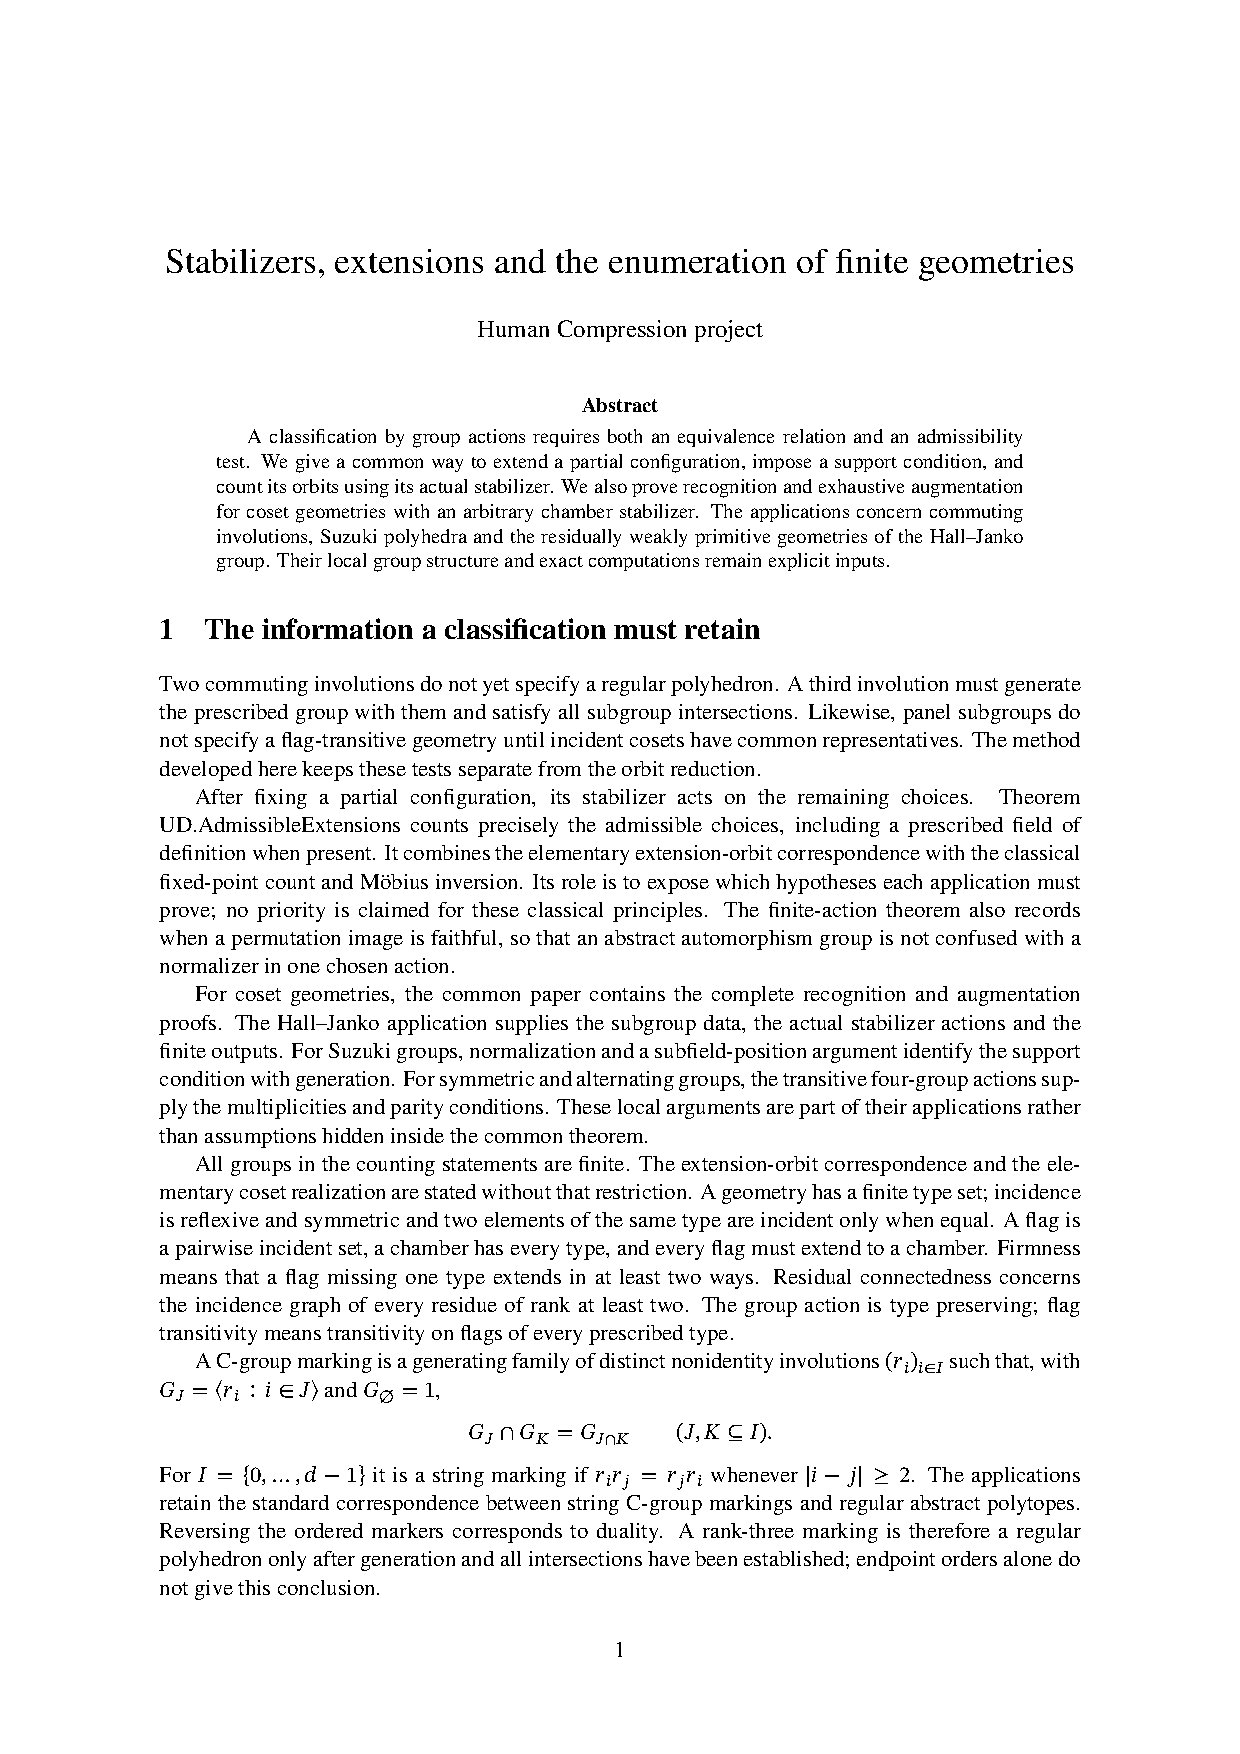
\includepdf[pages=-,pagecommand={},addtotoc={1,subsection,2,{Chapter 01: Common action and panel theory},proof01}]{proofs/01.pdf}
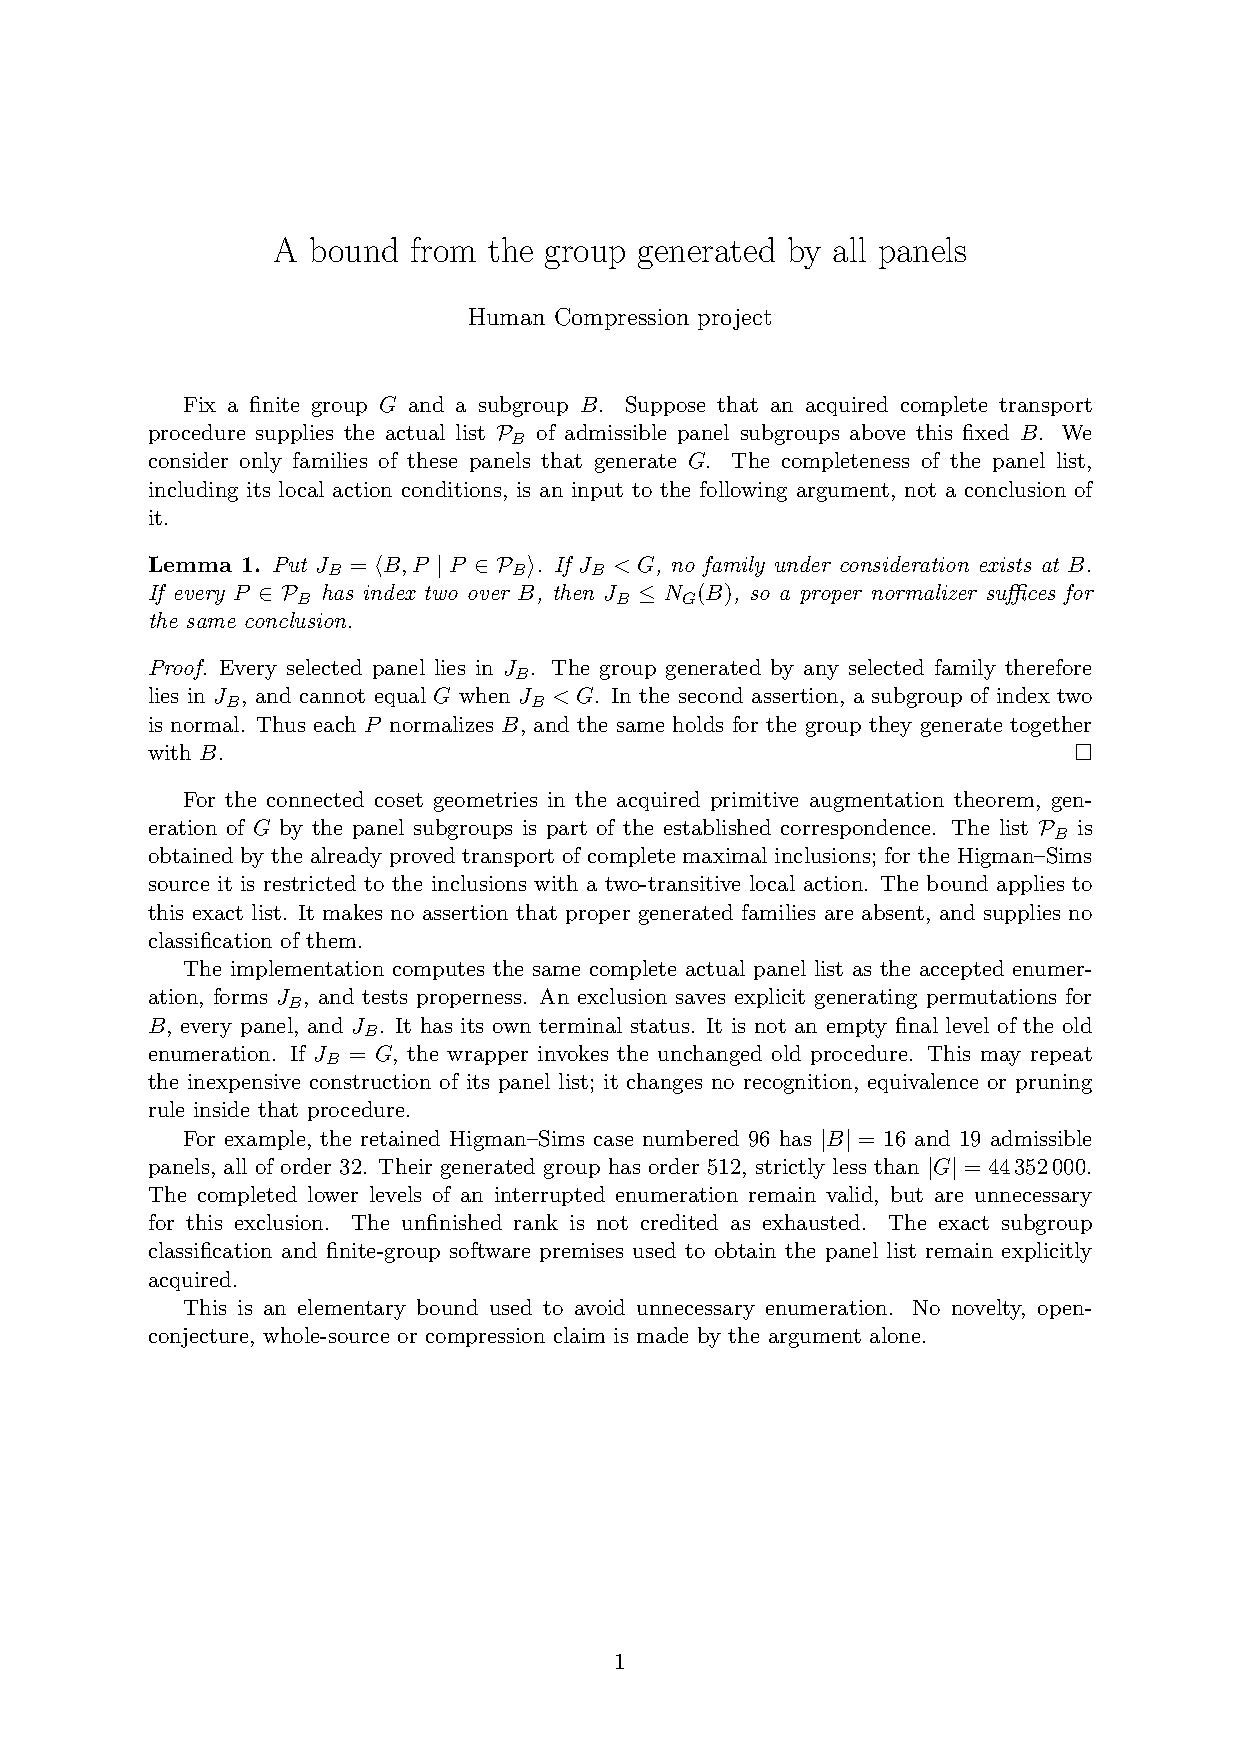
\includepdf[pages=-,pagecommand={},addtotoc={1,subsection,2,{Chapter 02: Generation by all admissible panels},proof02}]{proofs/02.pdf}
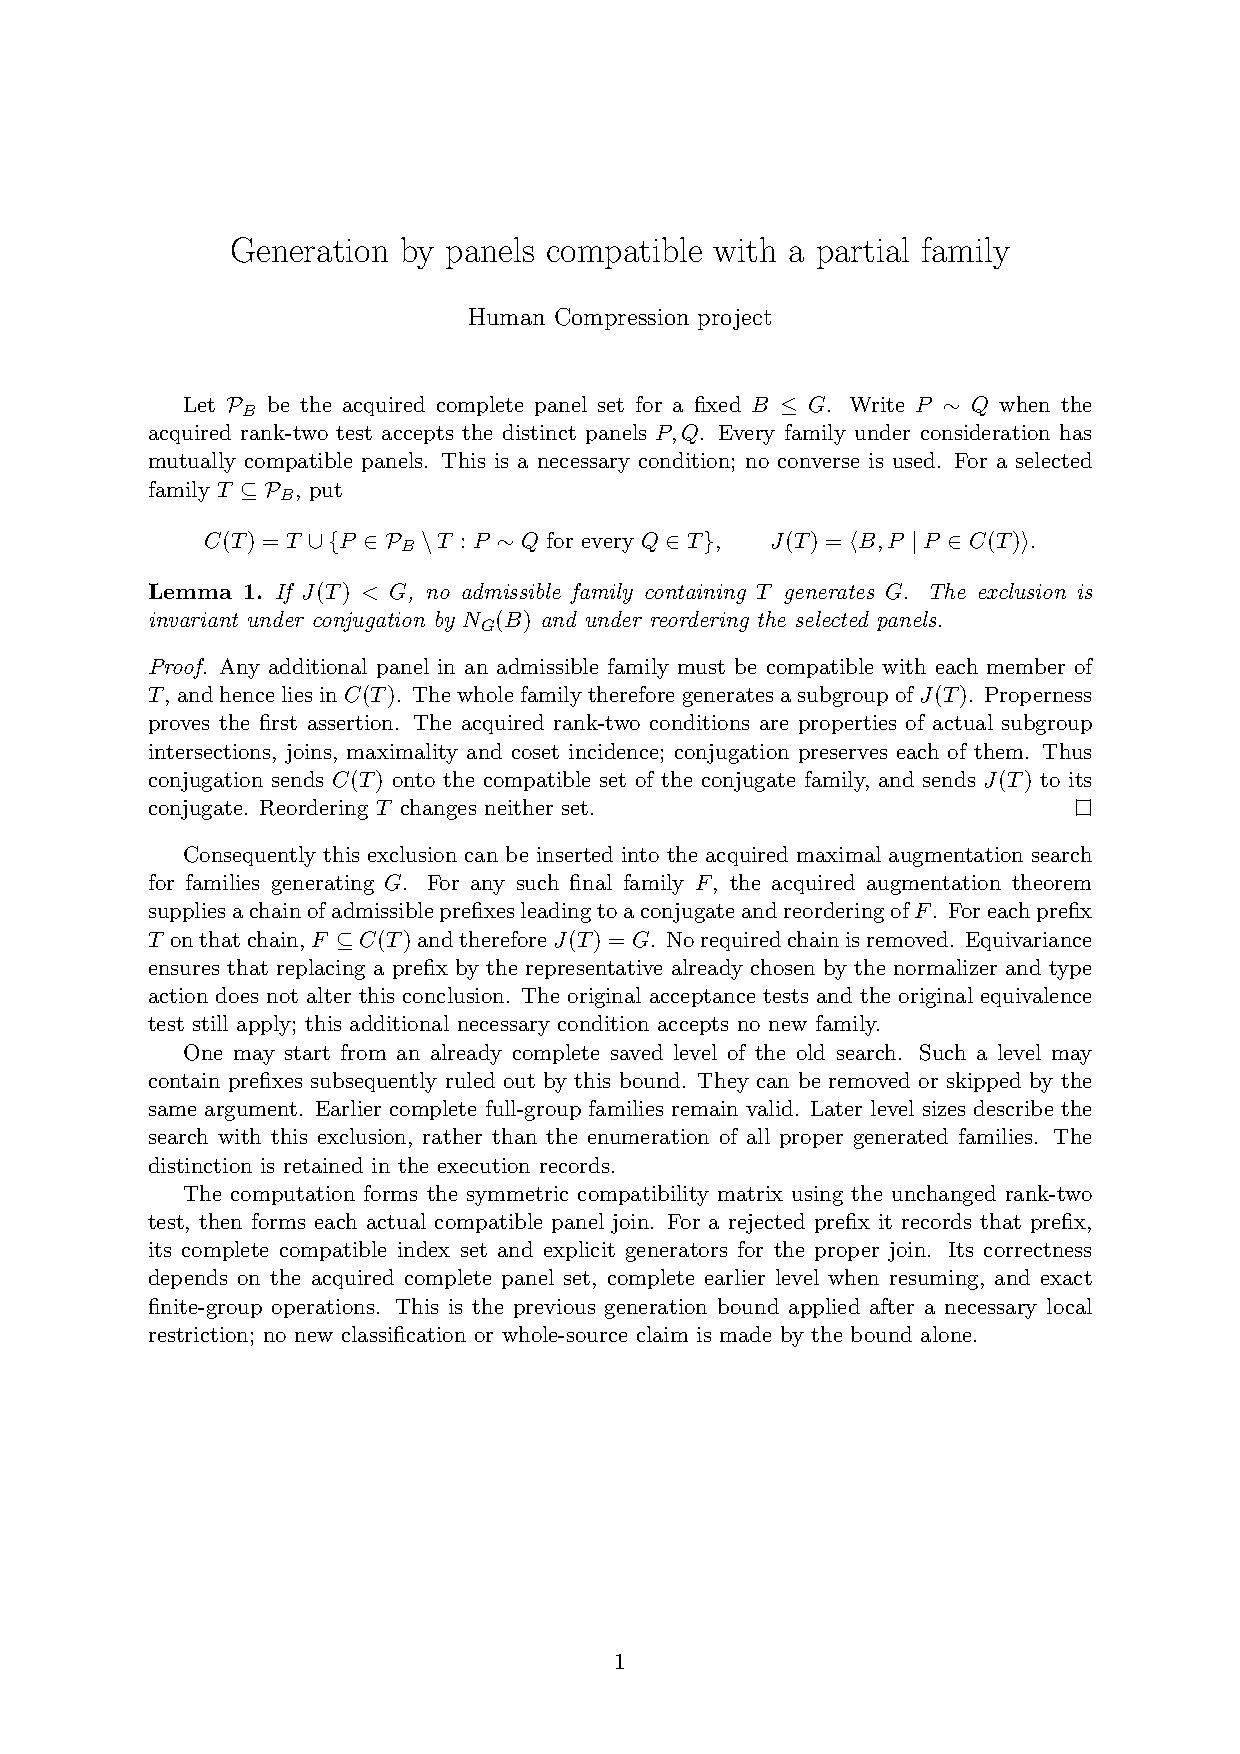
\includepdf[pages=-,pagecommand={},addtotoc={1,subsection,2,{Chapter 03: Compatible-panel generation},proof03}]{proofs/03.pdf}
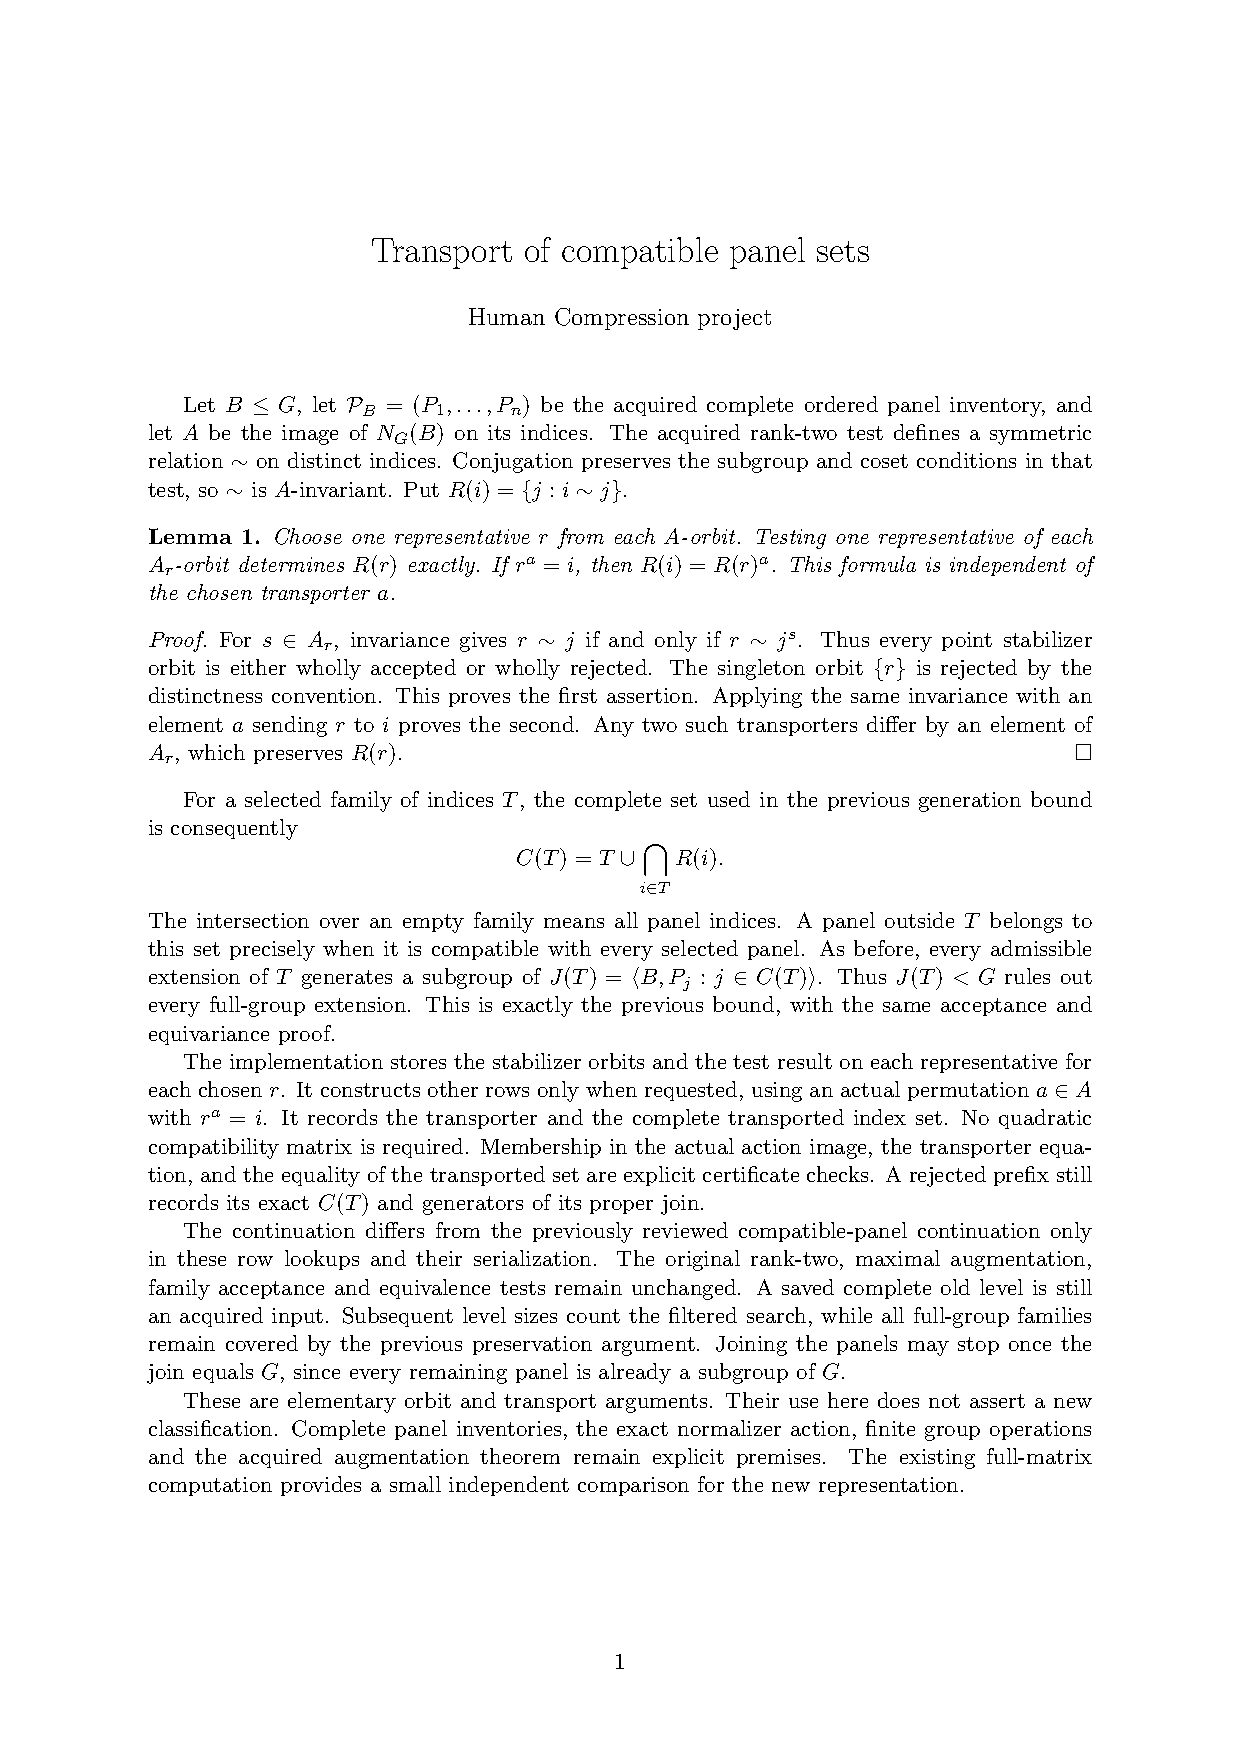
\includepdf[pages=-,pagecommand={},addtotoc={1,subsection,2,{Chapter 04: Transport of compatible panel sets},proof04}]{proofs/04.pdf}
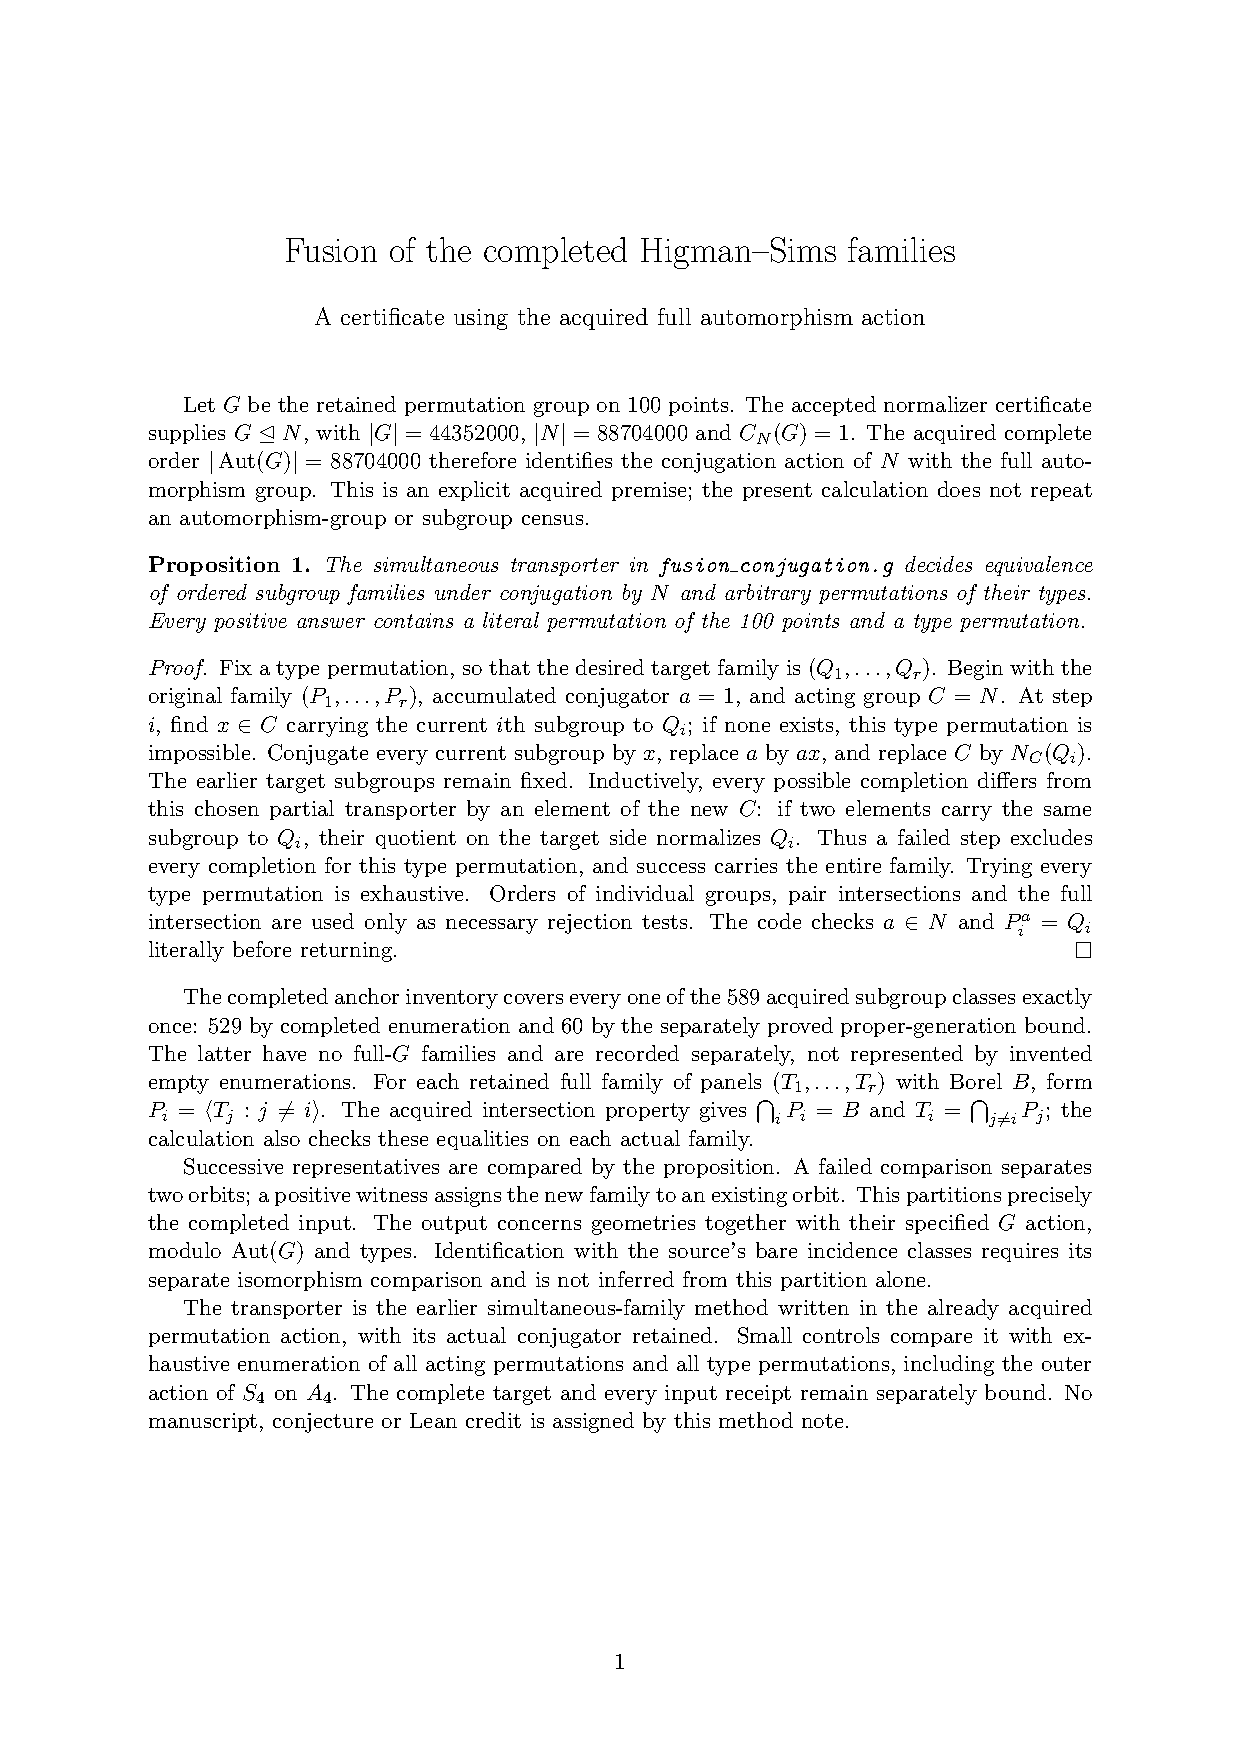
\includepdf[pages=-,pagecommand={},addtotoc={1,subsection,2,{Chapter 05: Fusion under full group automorphisms},proof05}]{proofs/05.pdf}
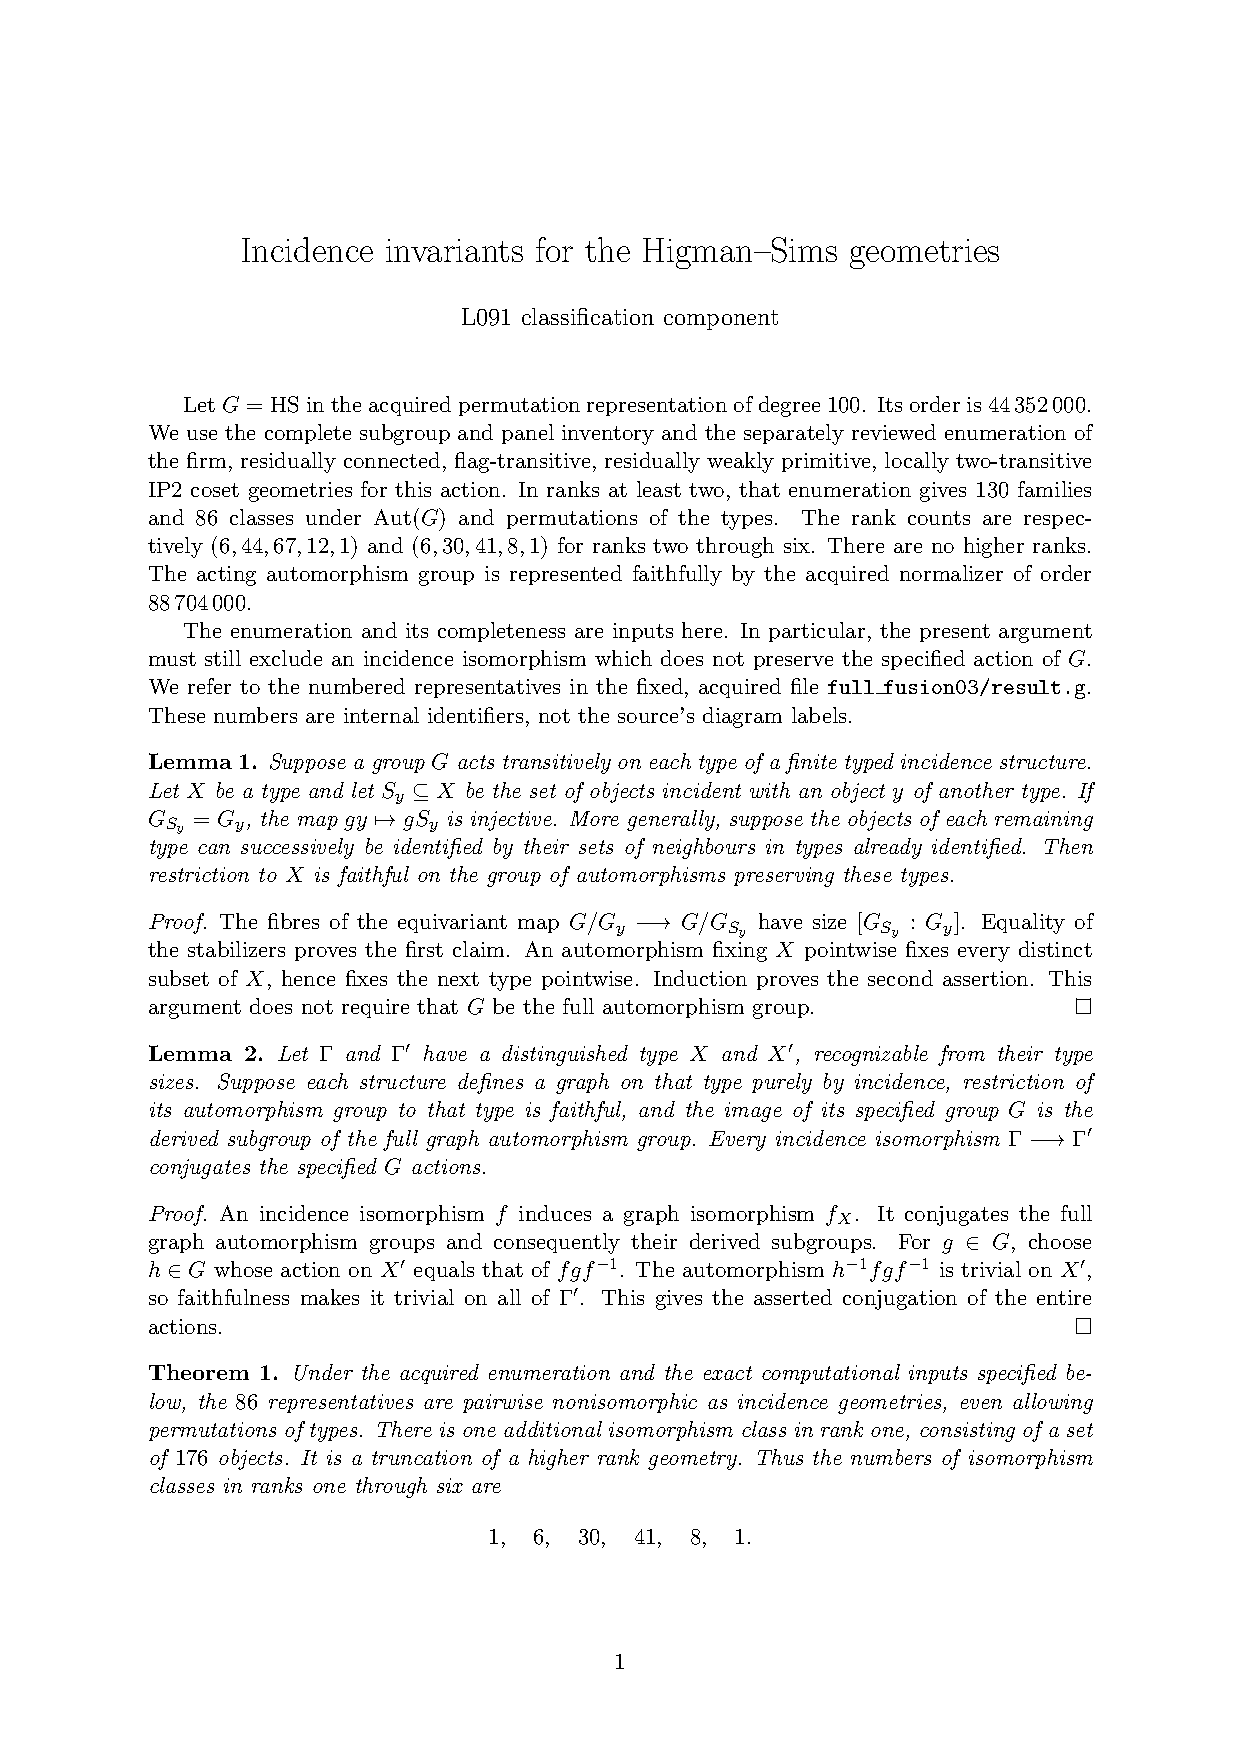
\includepdf[pages=-,pagecommand={},addtotoc={1,subsection,2,{Chapter 06: Bare incidence separation and rank one},proof06}]{proofs/06.pdf}
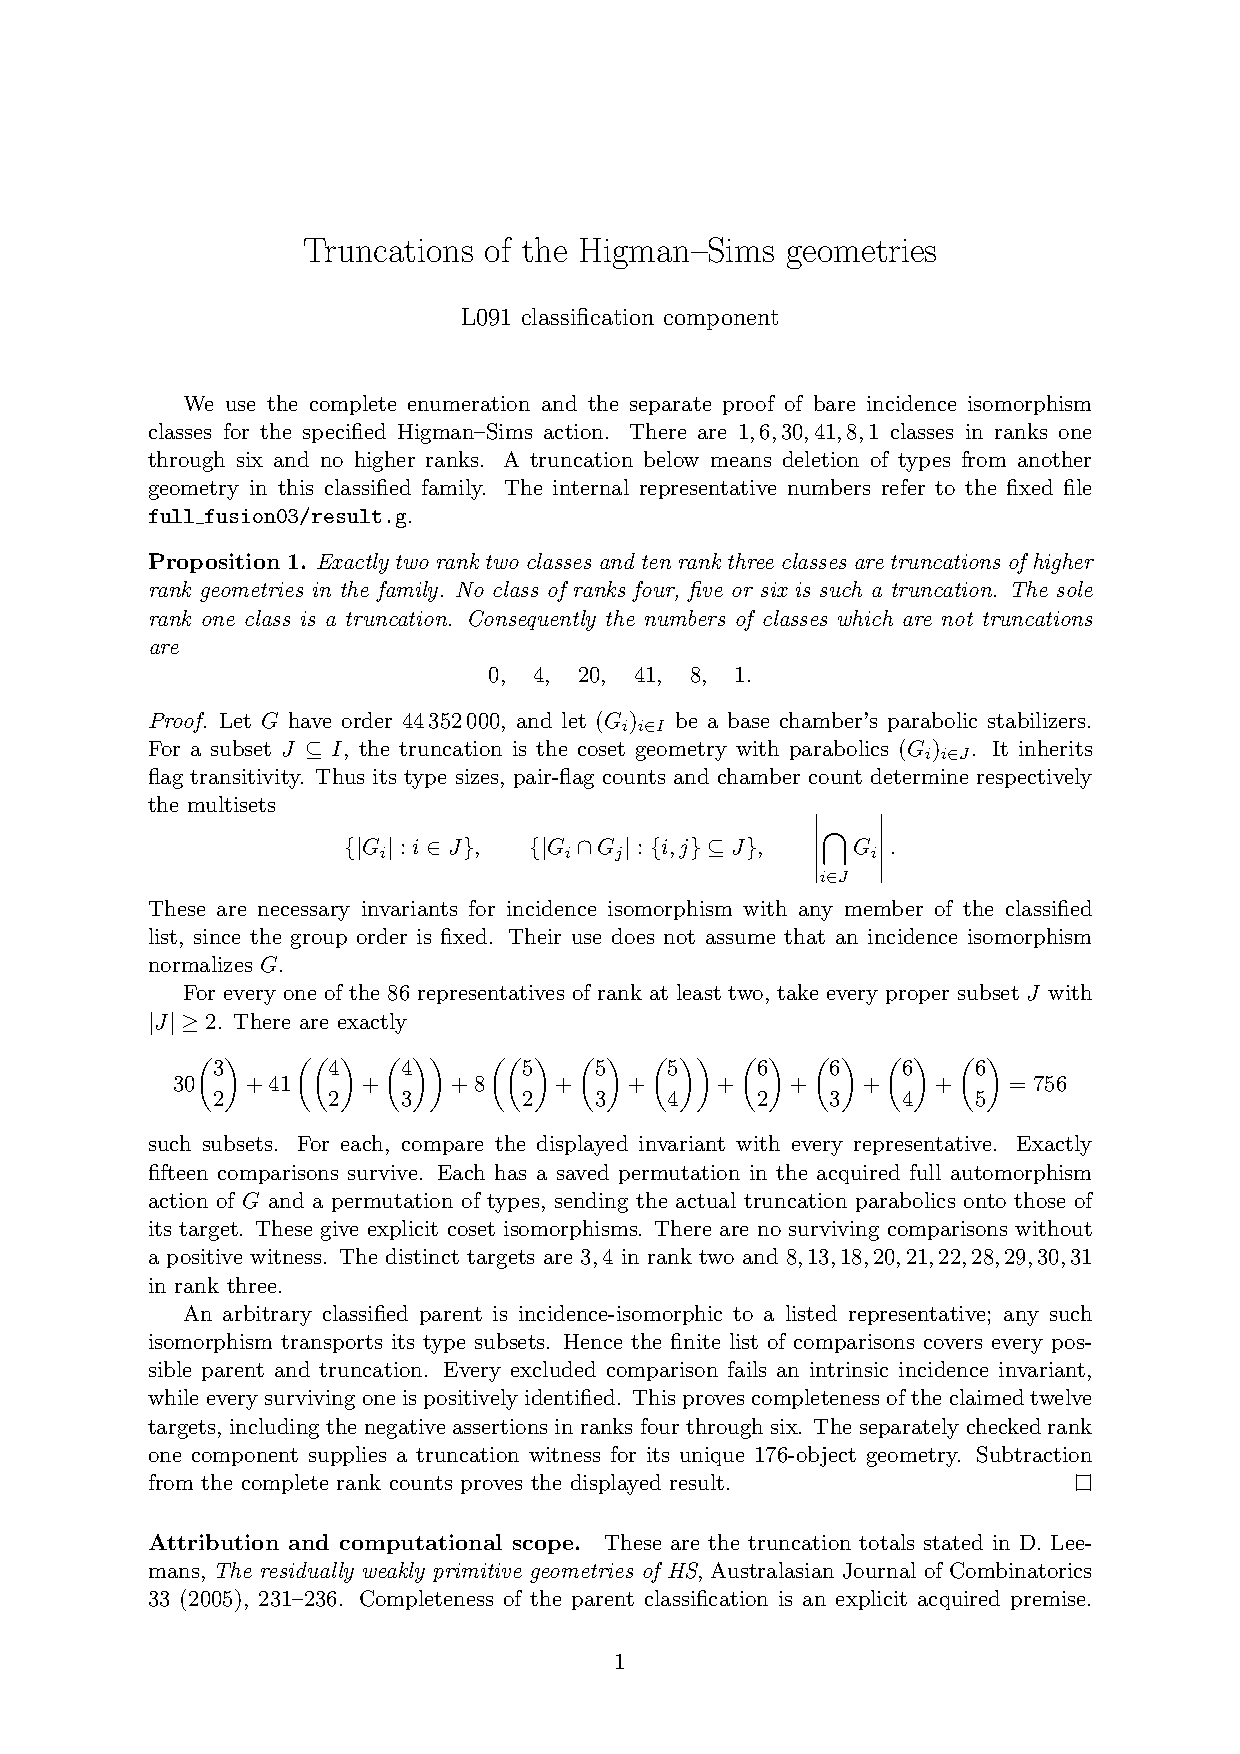
\includepdf[pages=-,pagecommand={},addtotoc={1,subsection,2,{Chapter 07: All higher-rank truncations},proof07}]{proofs/07.pdf}
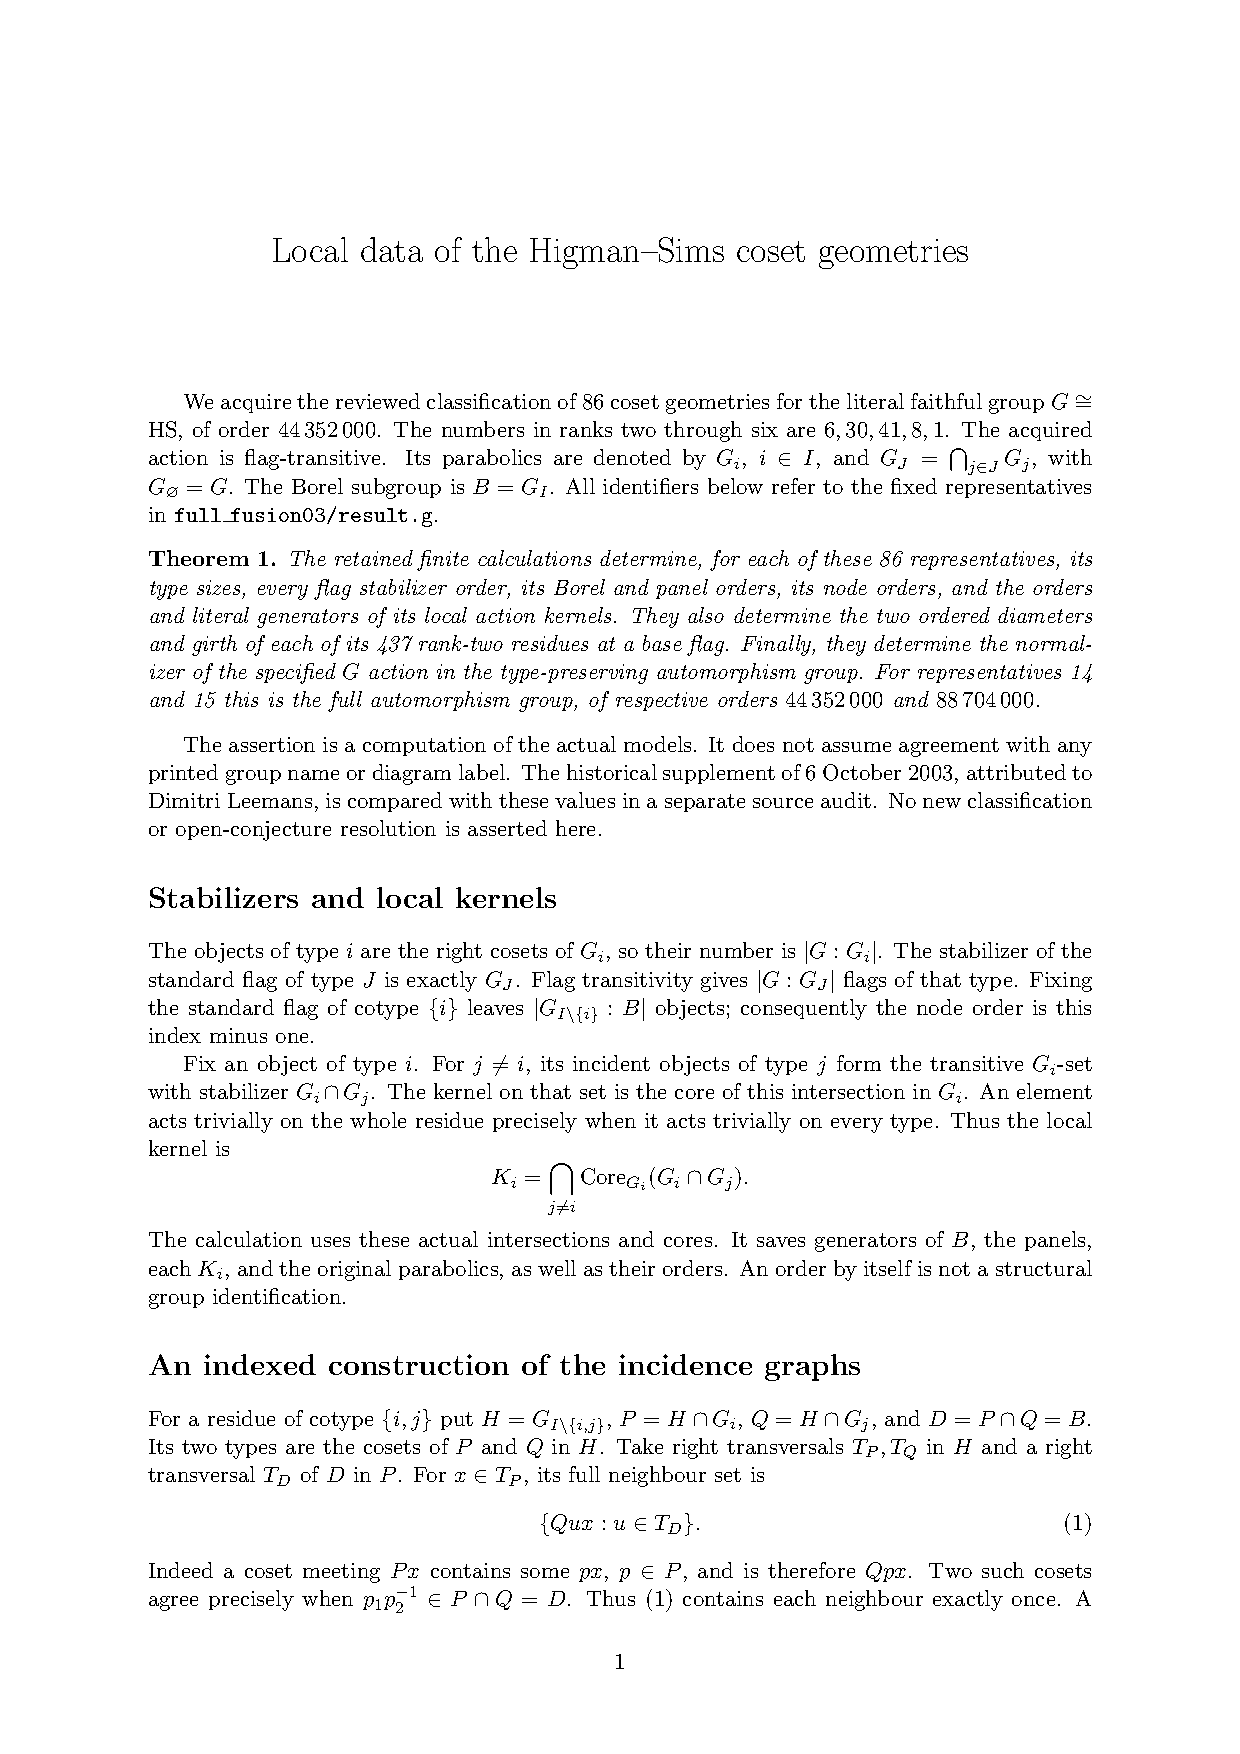
\includepdf[pages=-,pagecommand={},addtotoc={1,subsection,2,{Chapter 08: All local numerical data},proof08}]{proofs/08.pdf}
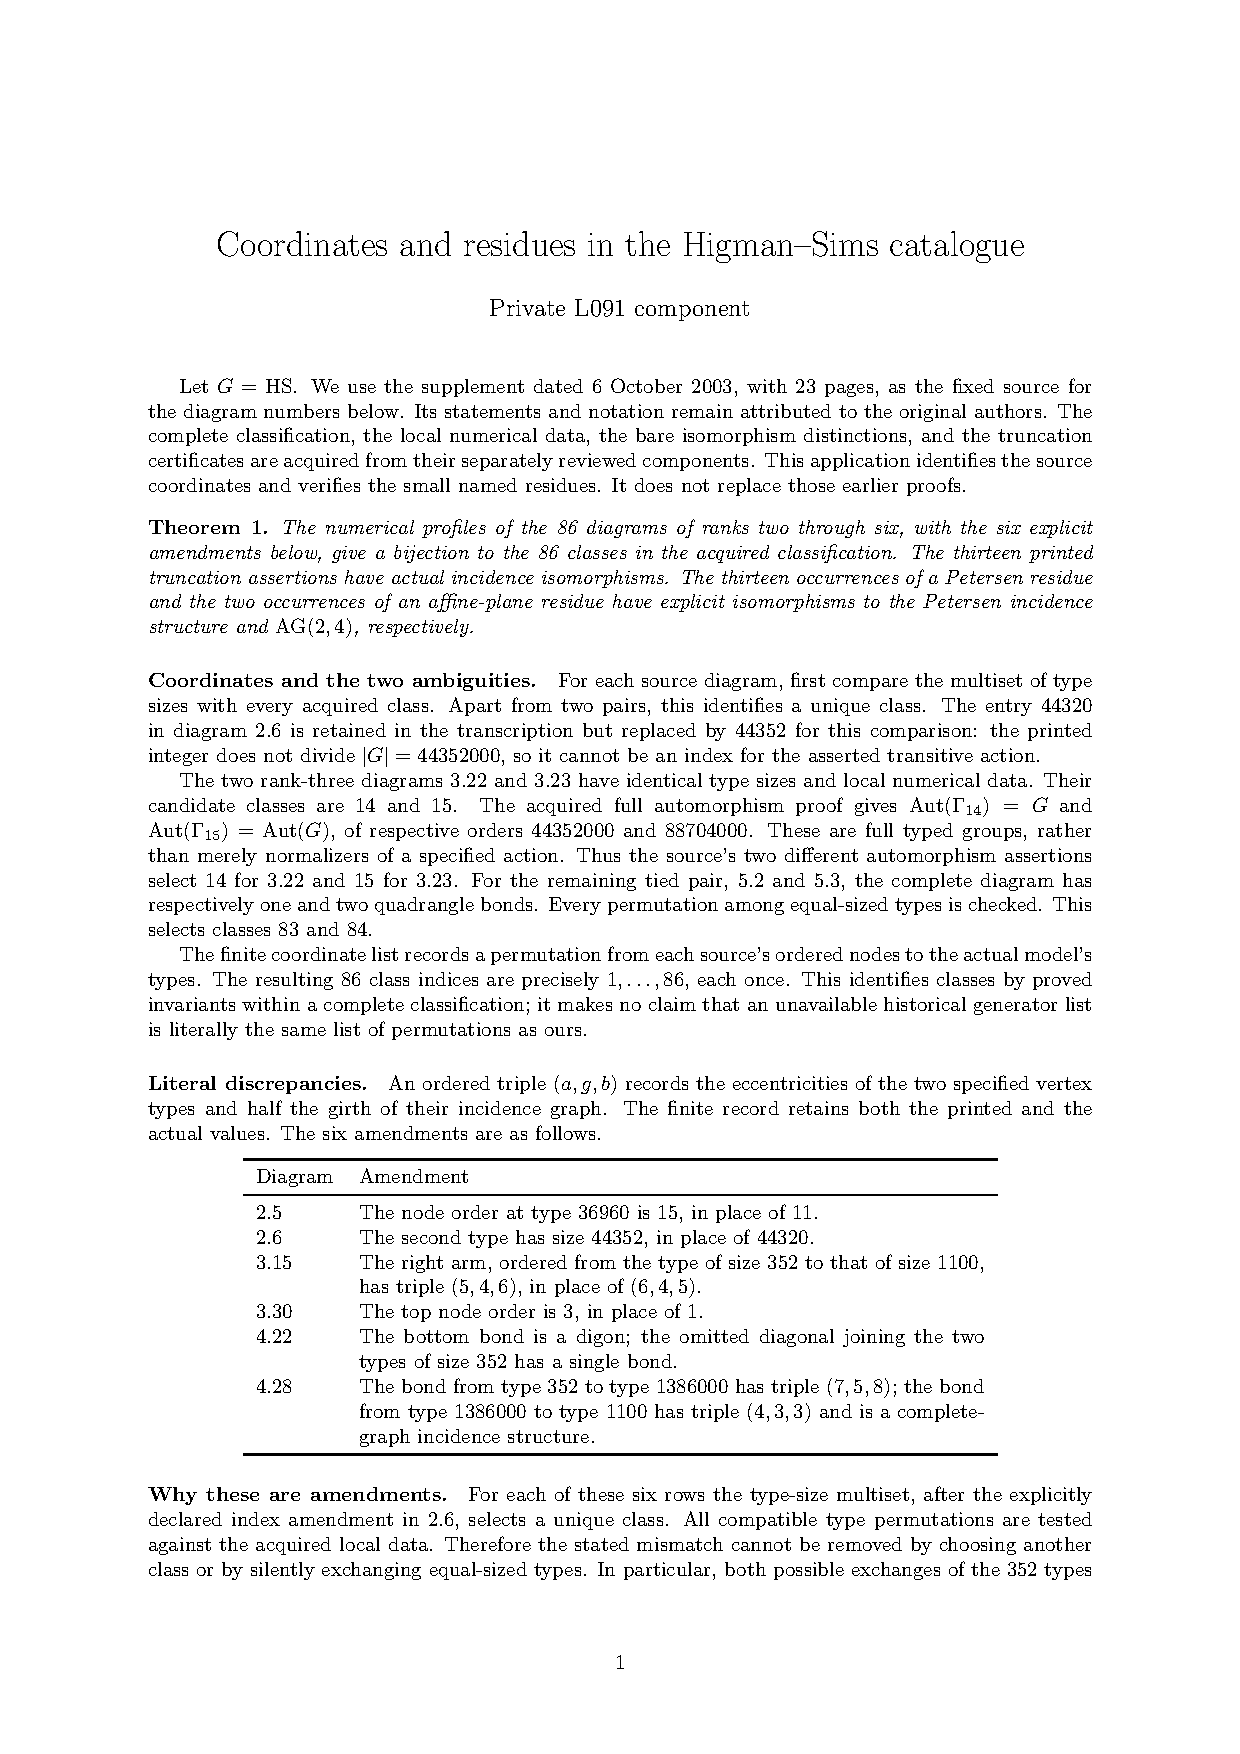
\includepdf[pages=-,pagecommand={},addtotoc={1,subsection,2,{Chapter 09: Source coordinates and named residues},proof09}]{proofs/09.pdf}
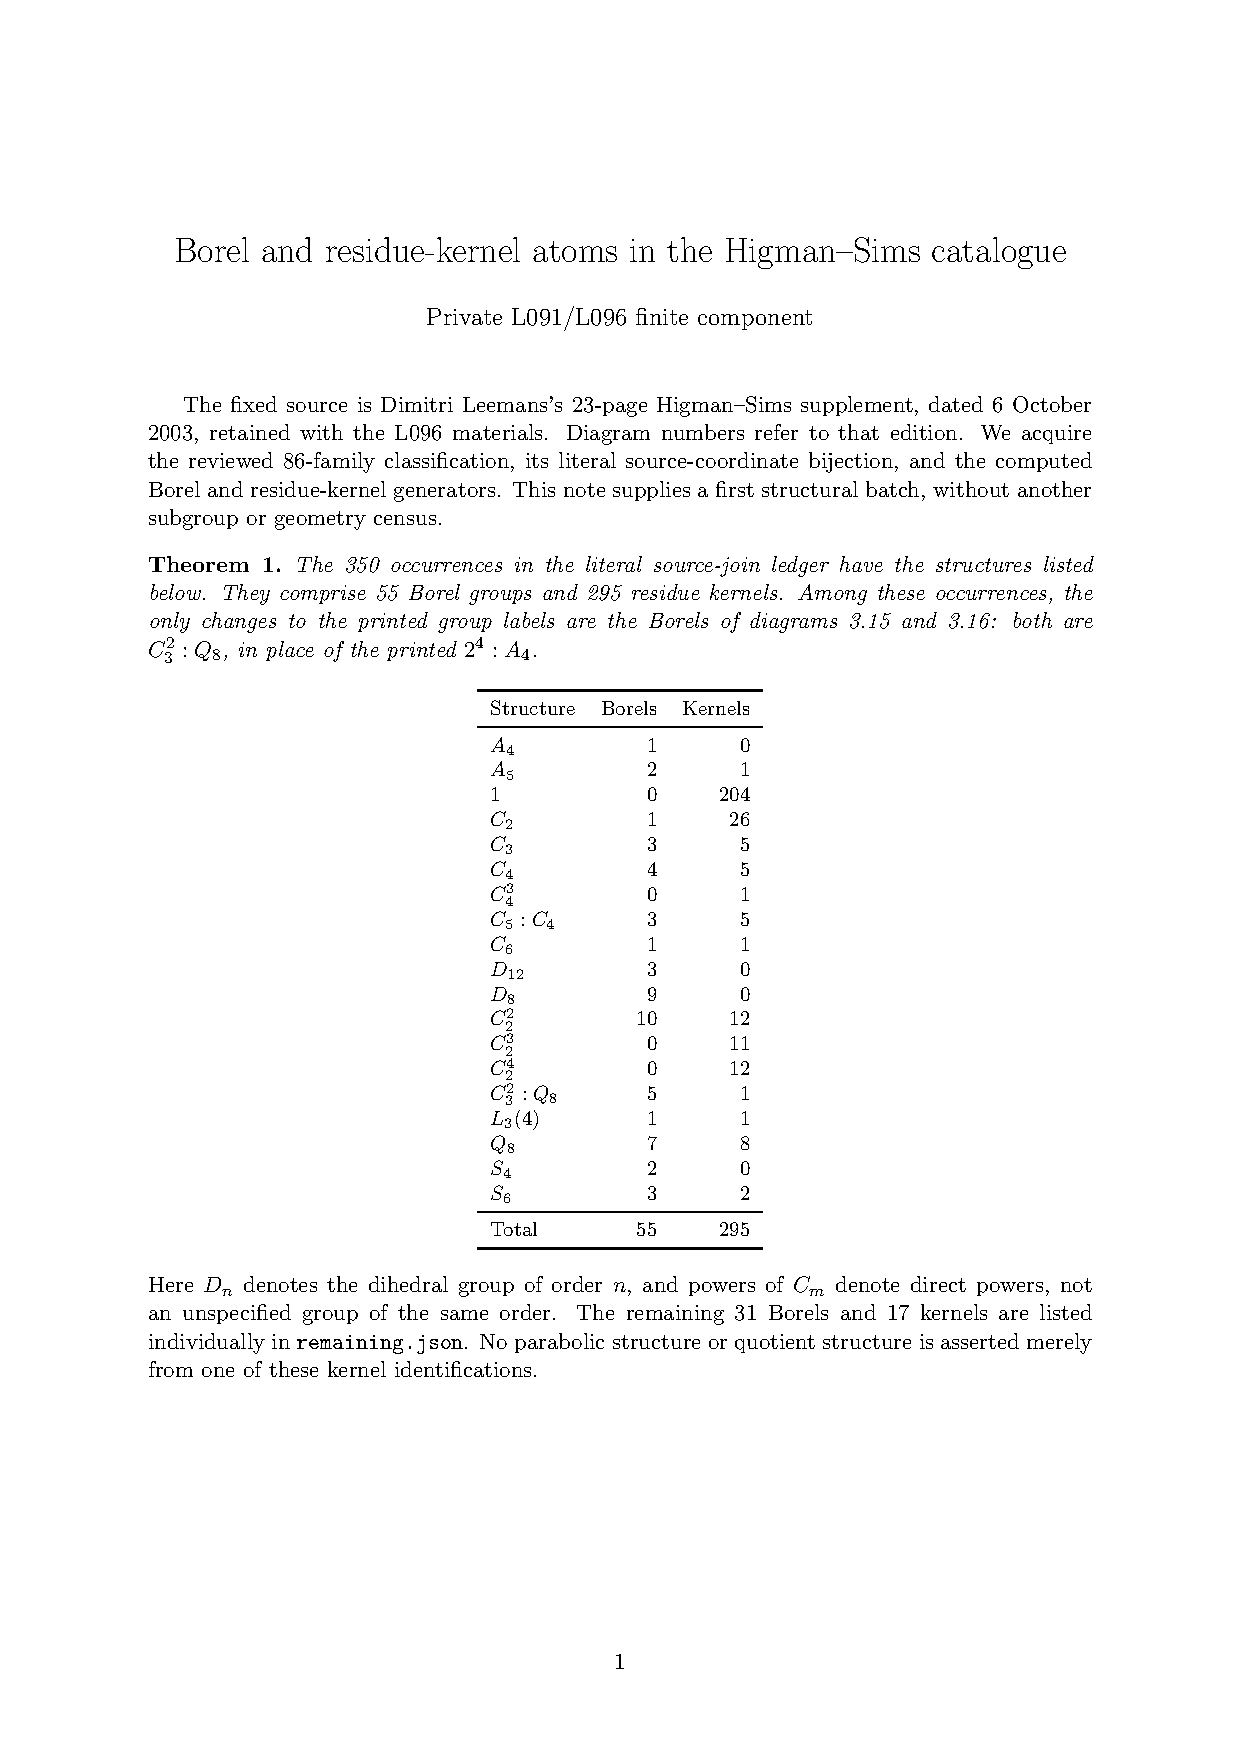
\includepdf[pages=-,pagecommand={},addtotoc={1,subsection,2,{Chapter 10: Elementary Borel and kernel structures},proof10}]{proofs/10.pdf}
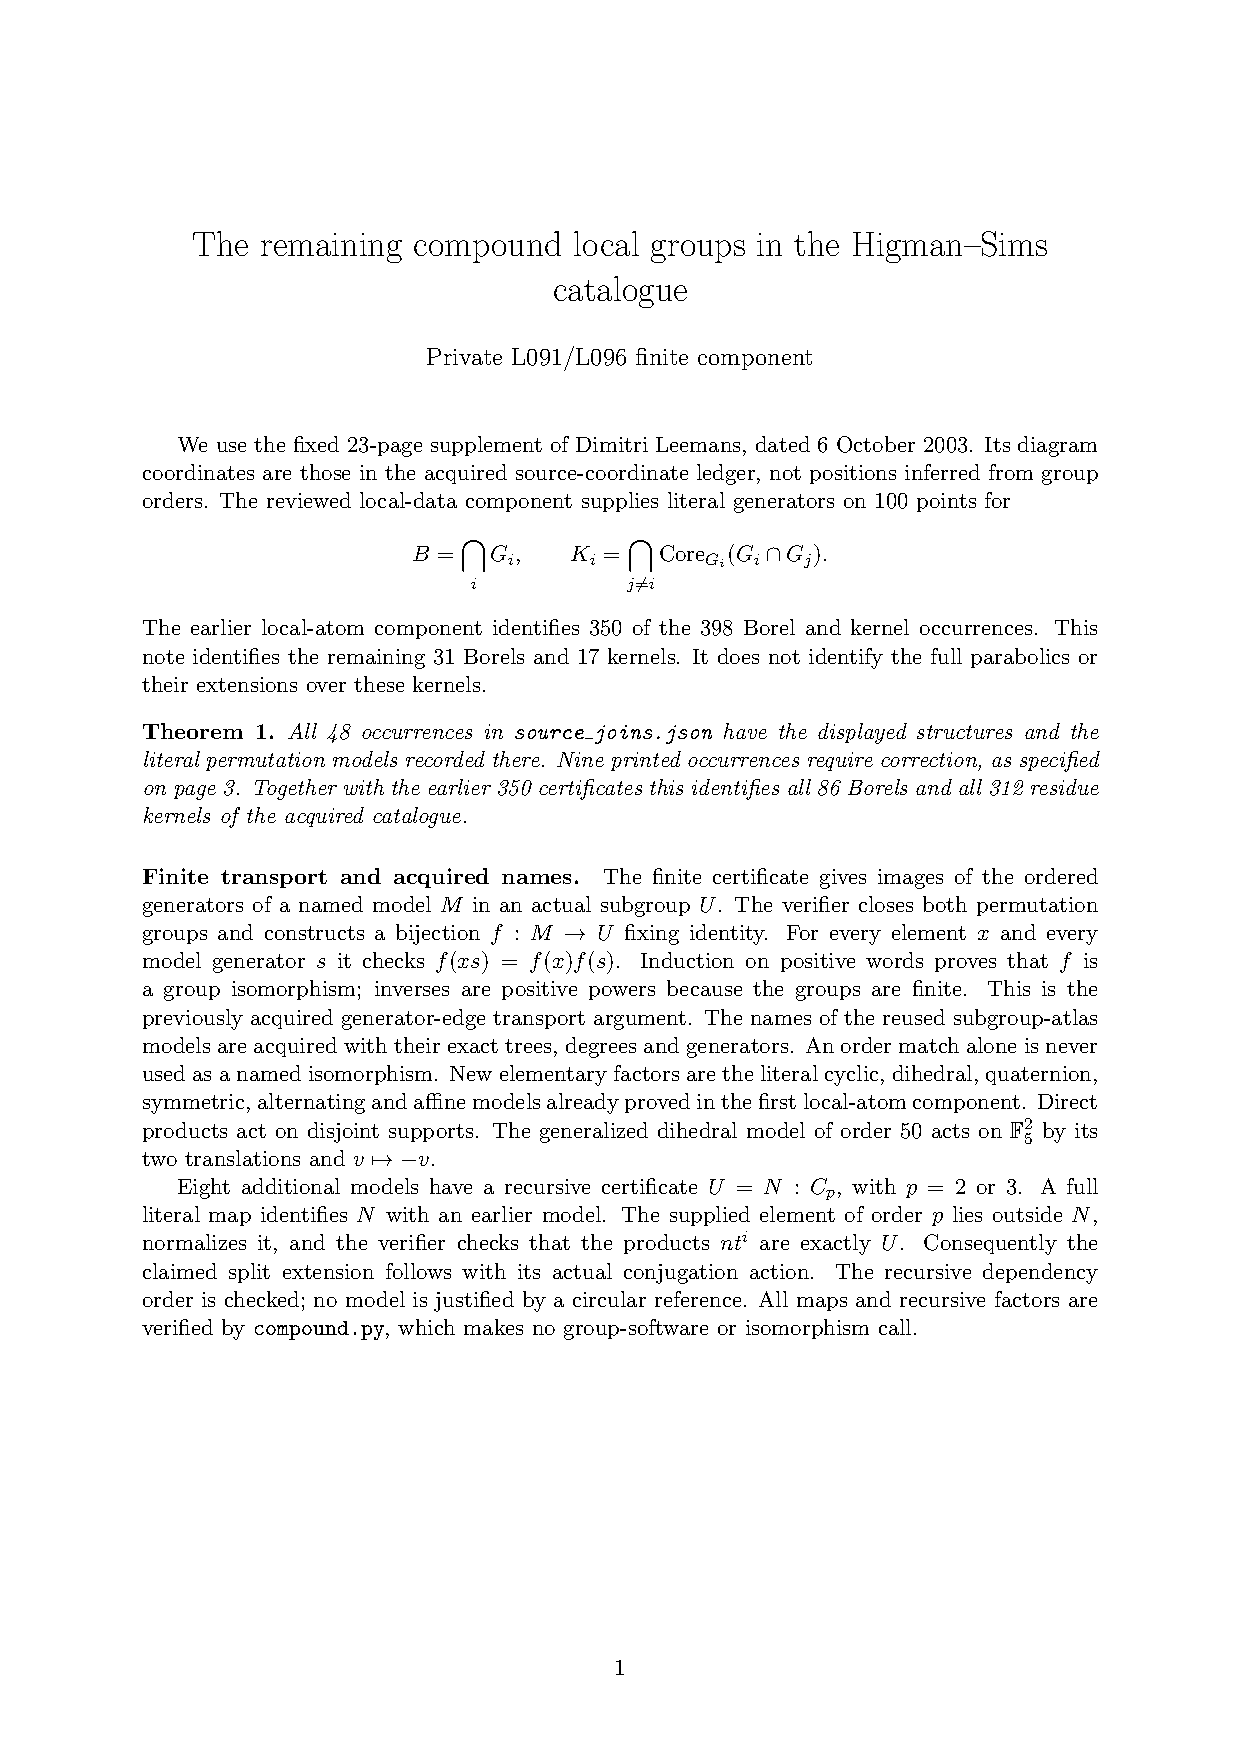
\includepdf[pages=-,pagecommand={},addtotoc={1,subsection,2,{Chapter 11: Compound Borel and kernel structures},proof11}]{proofs/11.pdf}
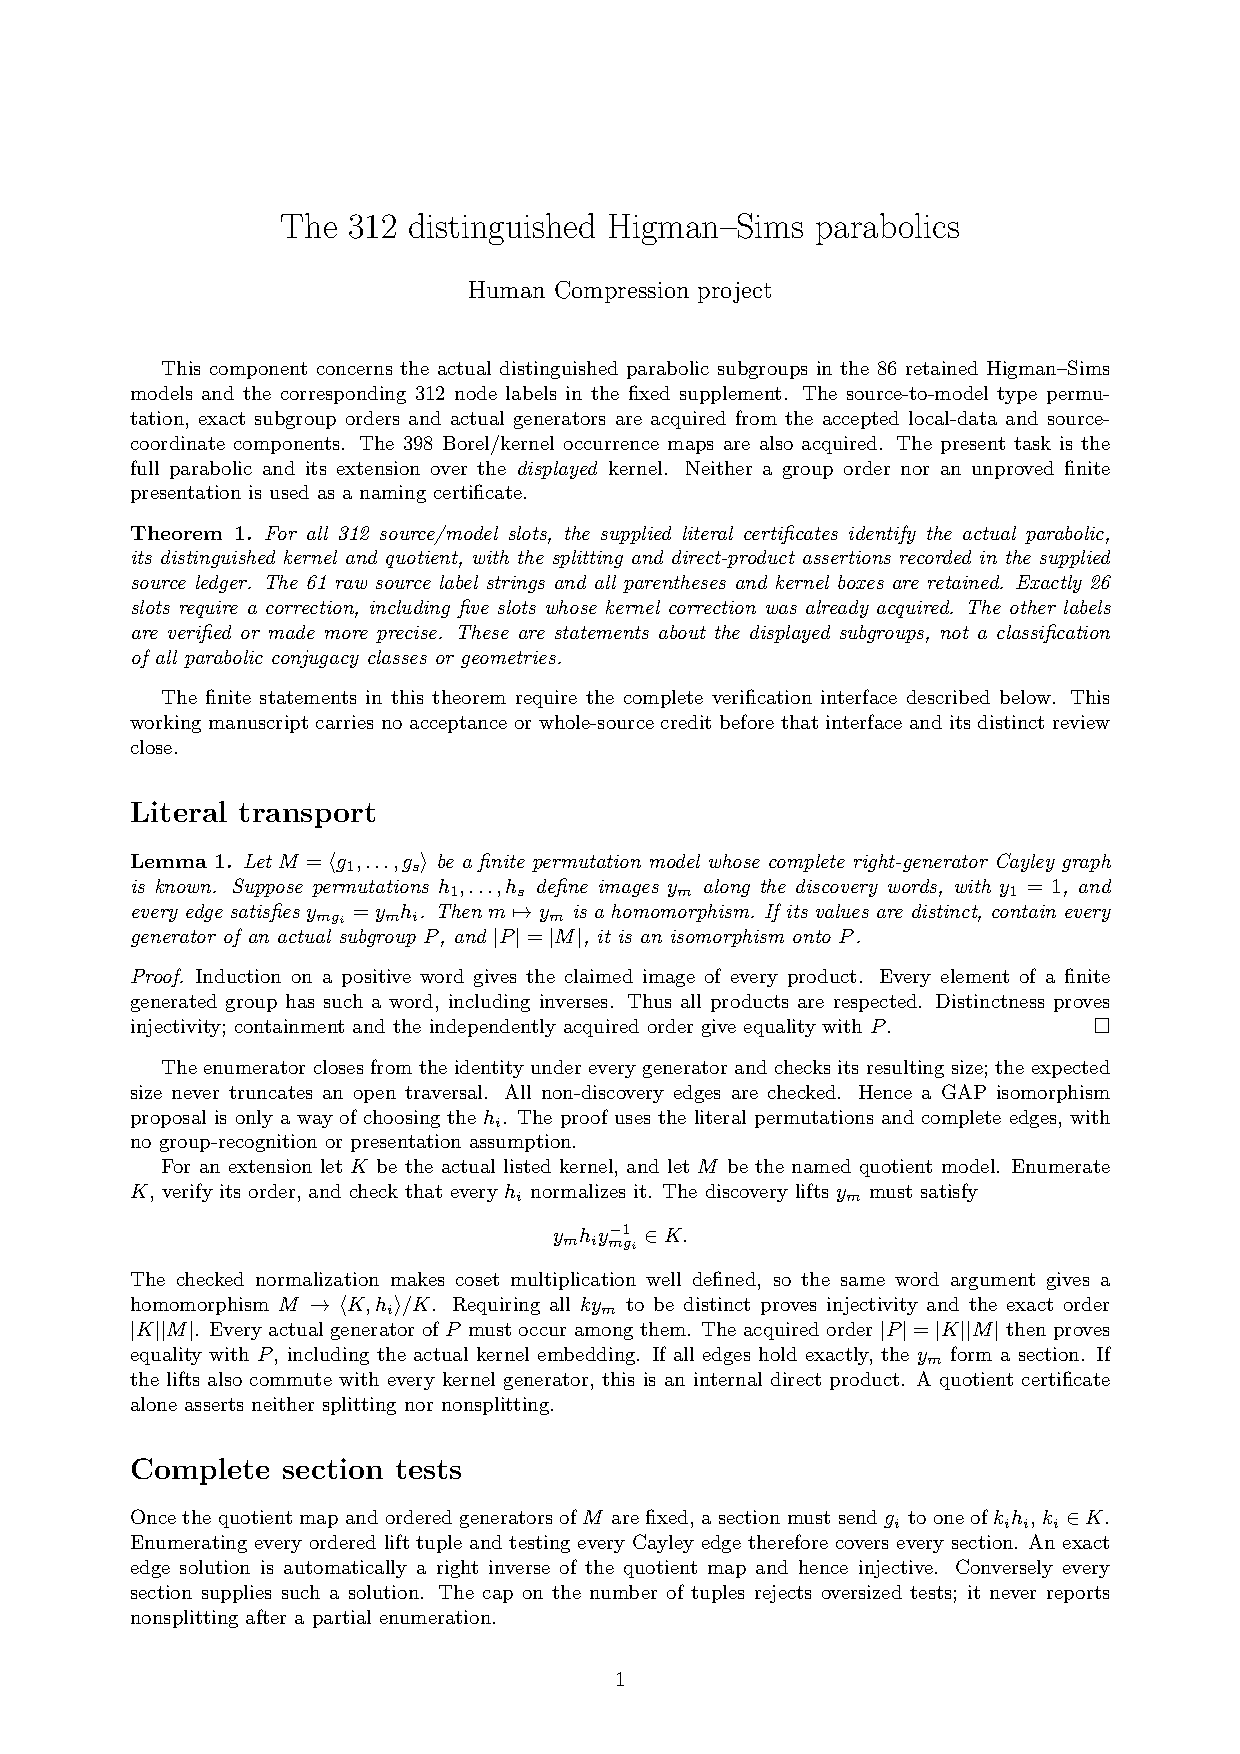
\includepdf[pages=-,pagecommand={},addtotoc={1,subsection,2,{Chapter 12: All distinguished parabolic structures},proof12}]{proofs/12.pdf}
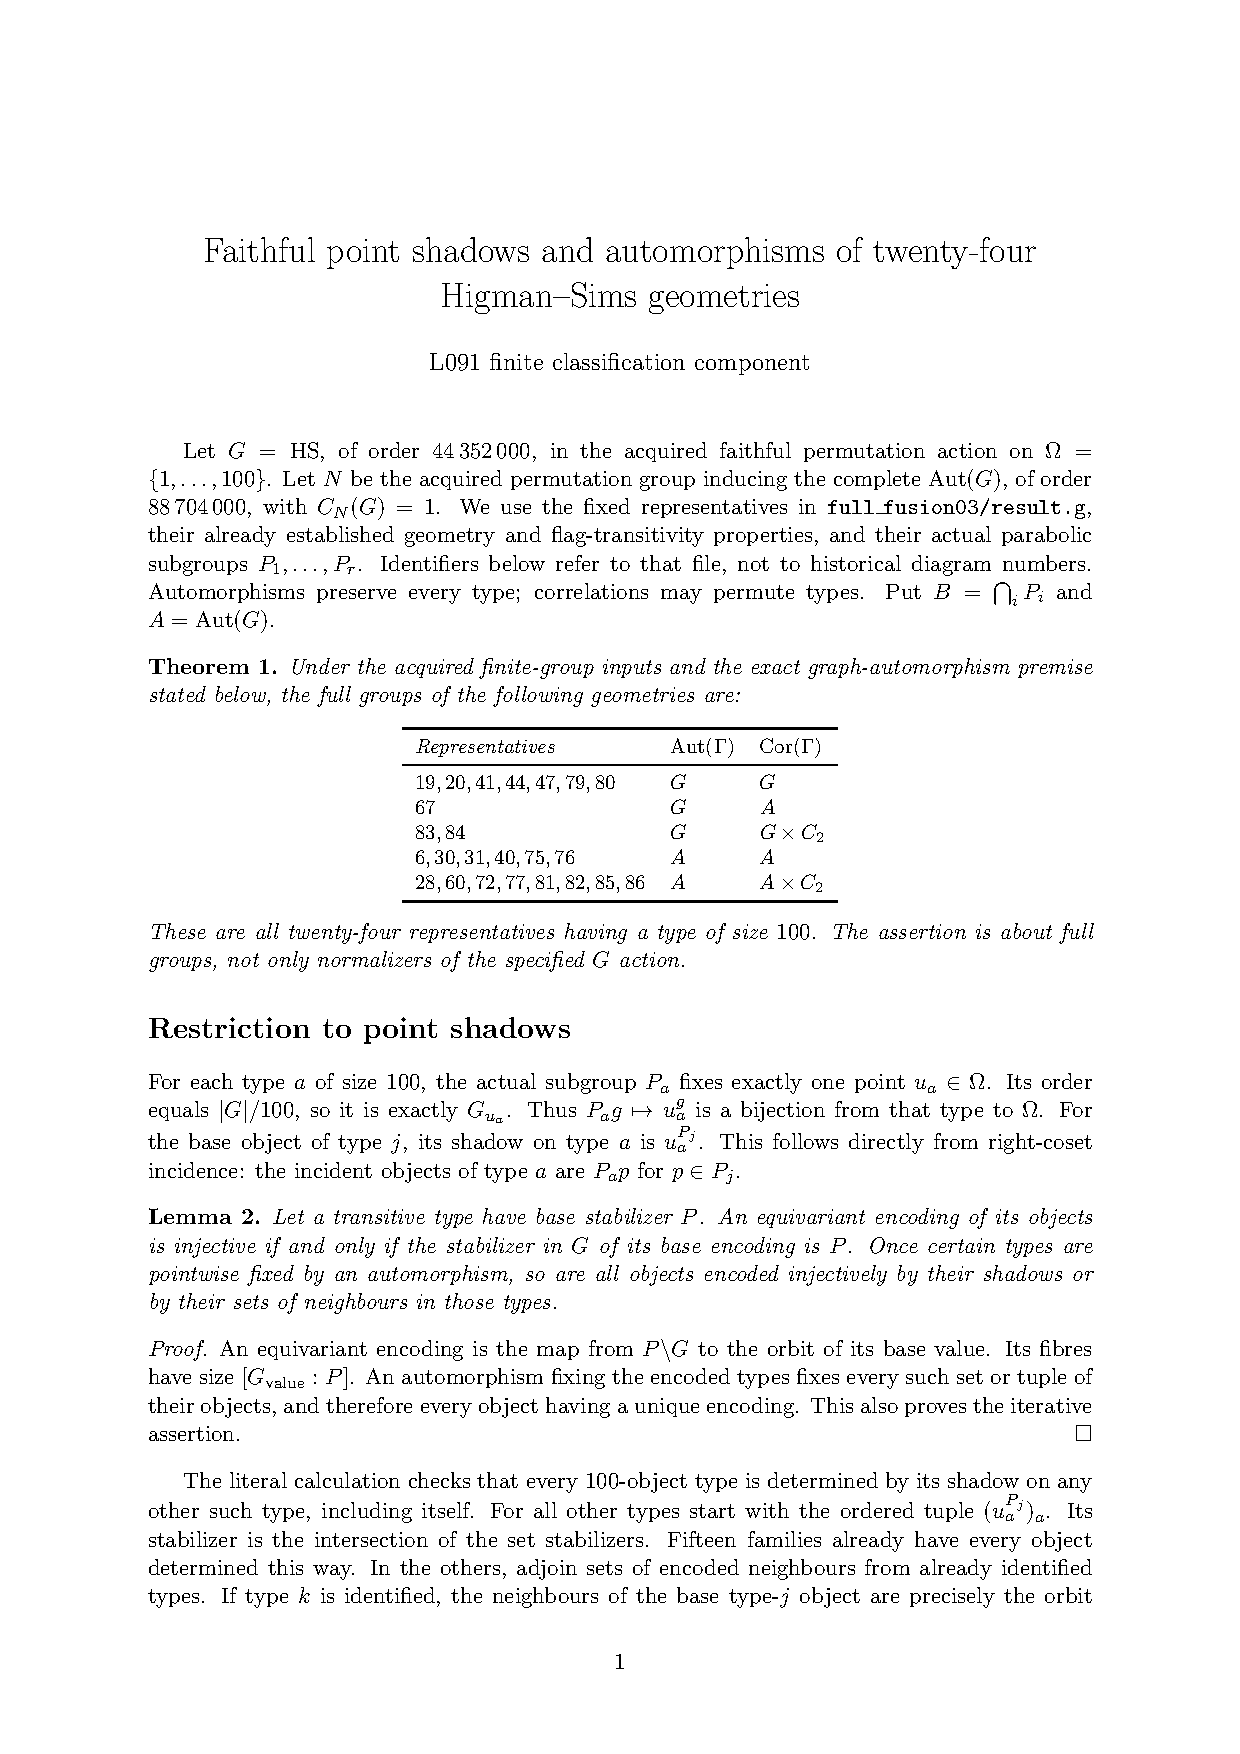
\includepdf[pages=-,pagecommand={},addtotoc={1,subsection,2,{Chapter 13: Groups from one hundred points},proof13}]{proofs/13.pdf}
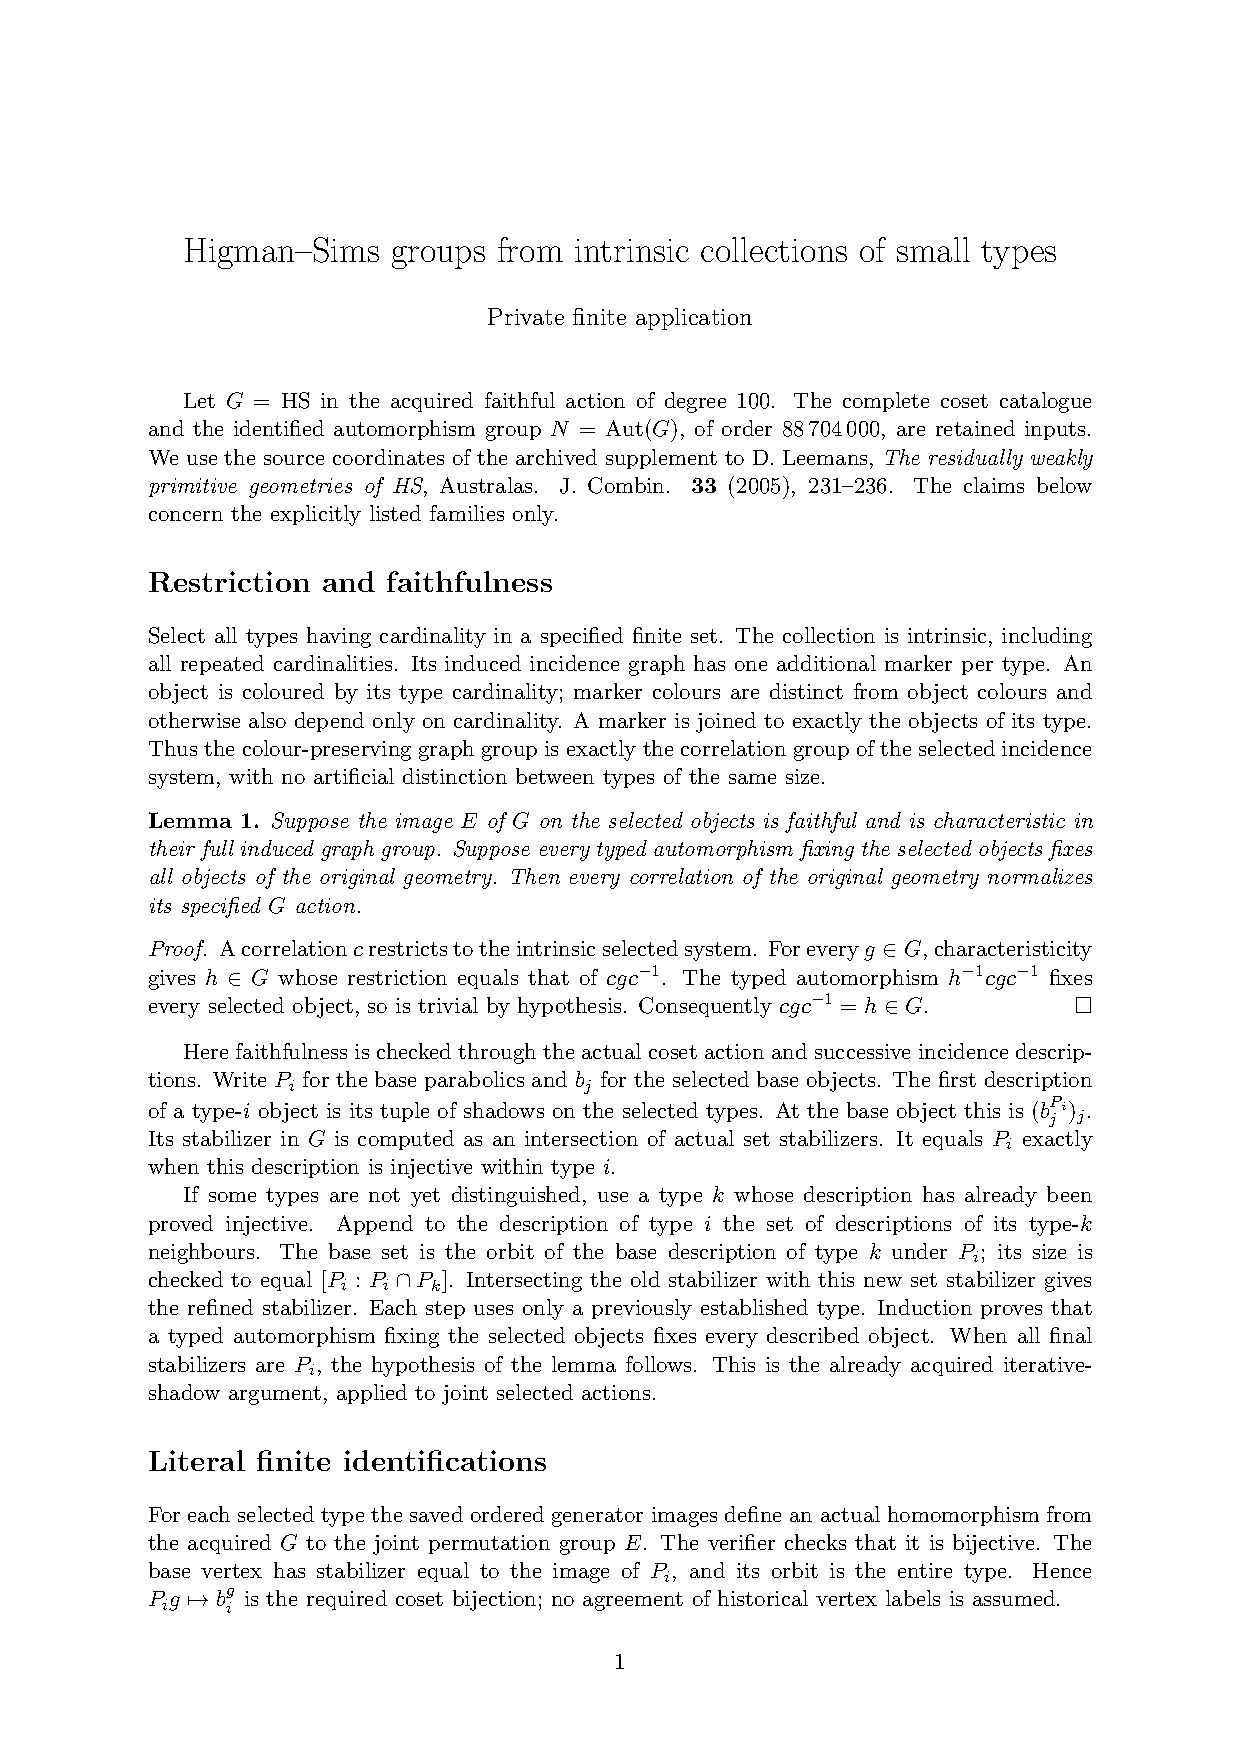
\includepdf[pages=-,pagecommand={},addtotoc={1,subsection,2,{Chapter 14: Nine groups from joint point actions},proof14}]{proofs/14.pdf}
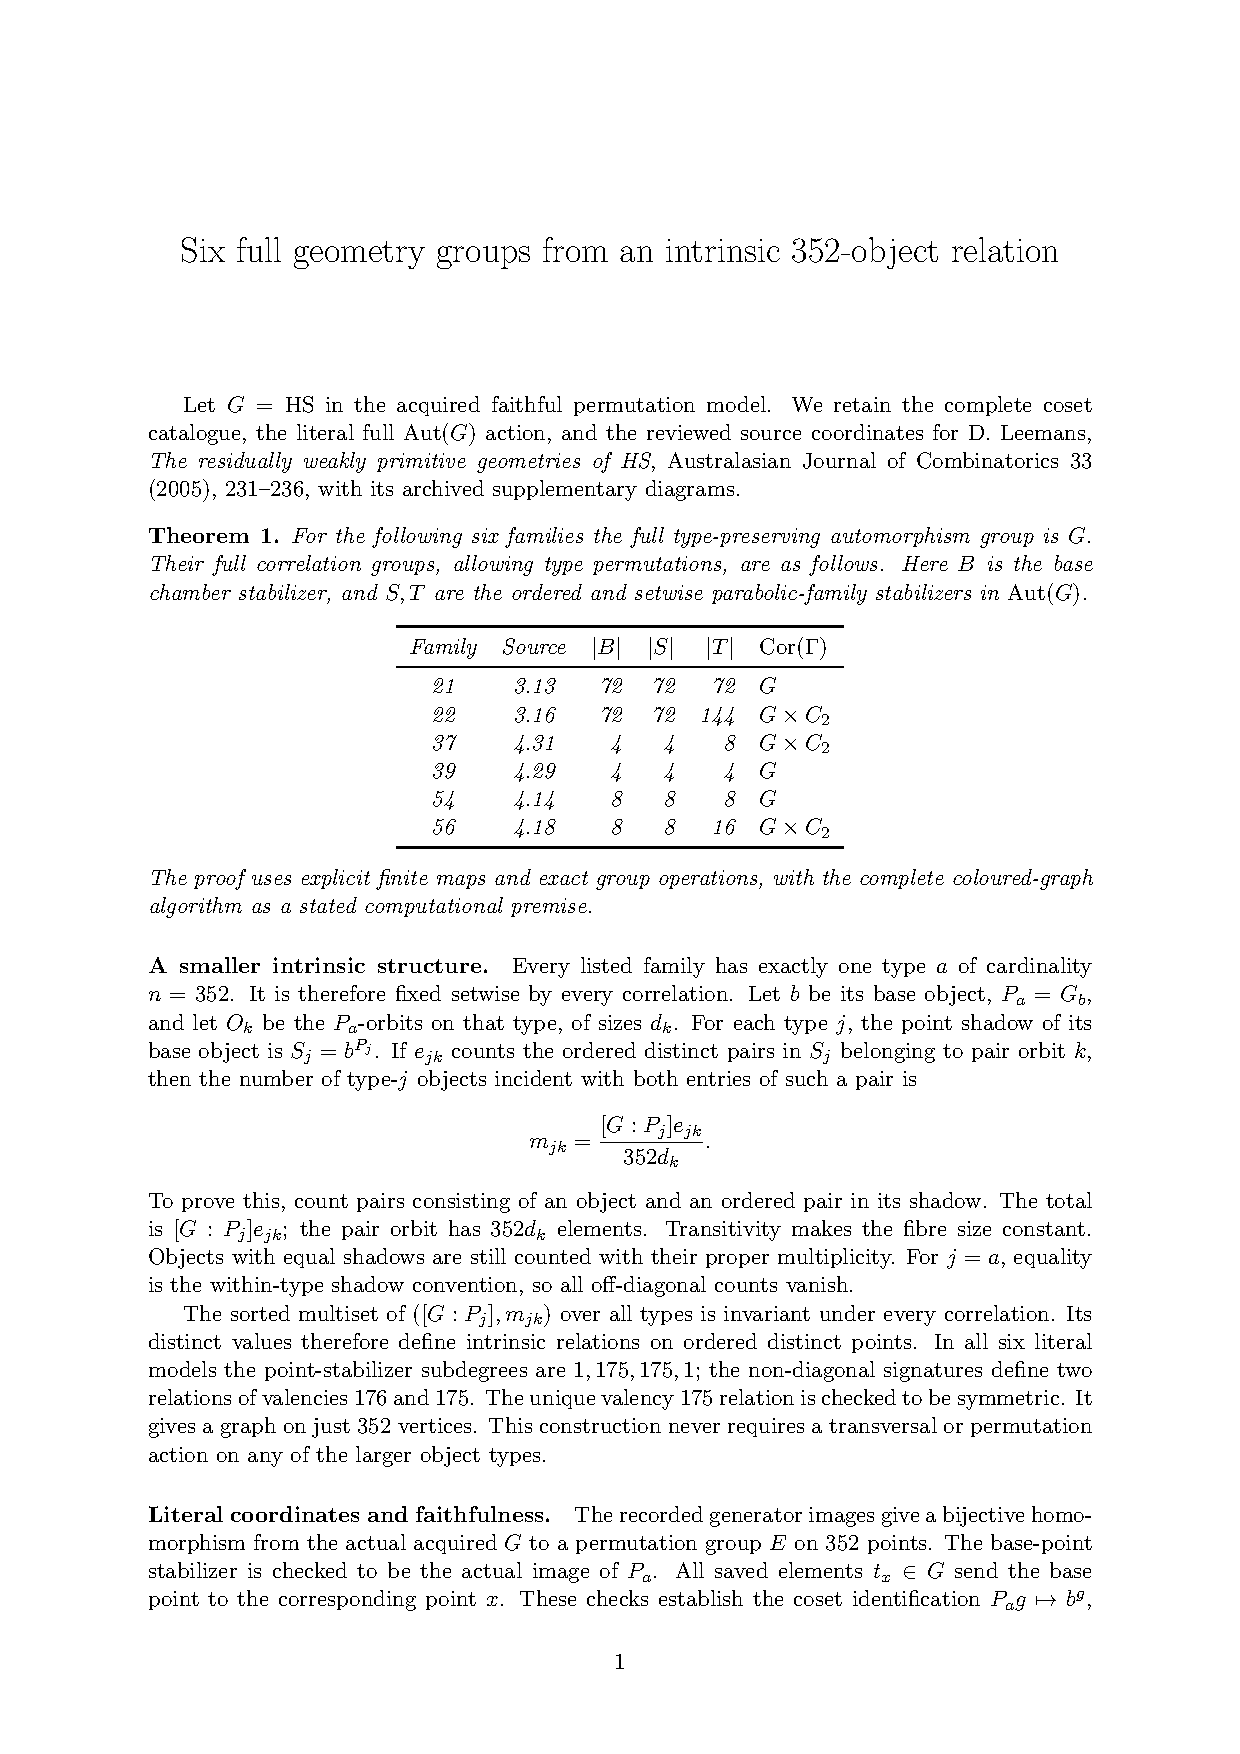
\includepdf[pages=-,pagecommand={},addtotoc={1,subsection,2,{Chapter 15: Six groups from 352 points},proof15}]{proofs/15.pdf}
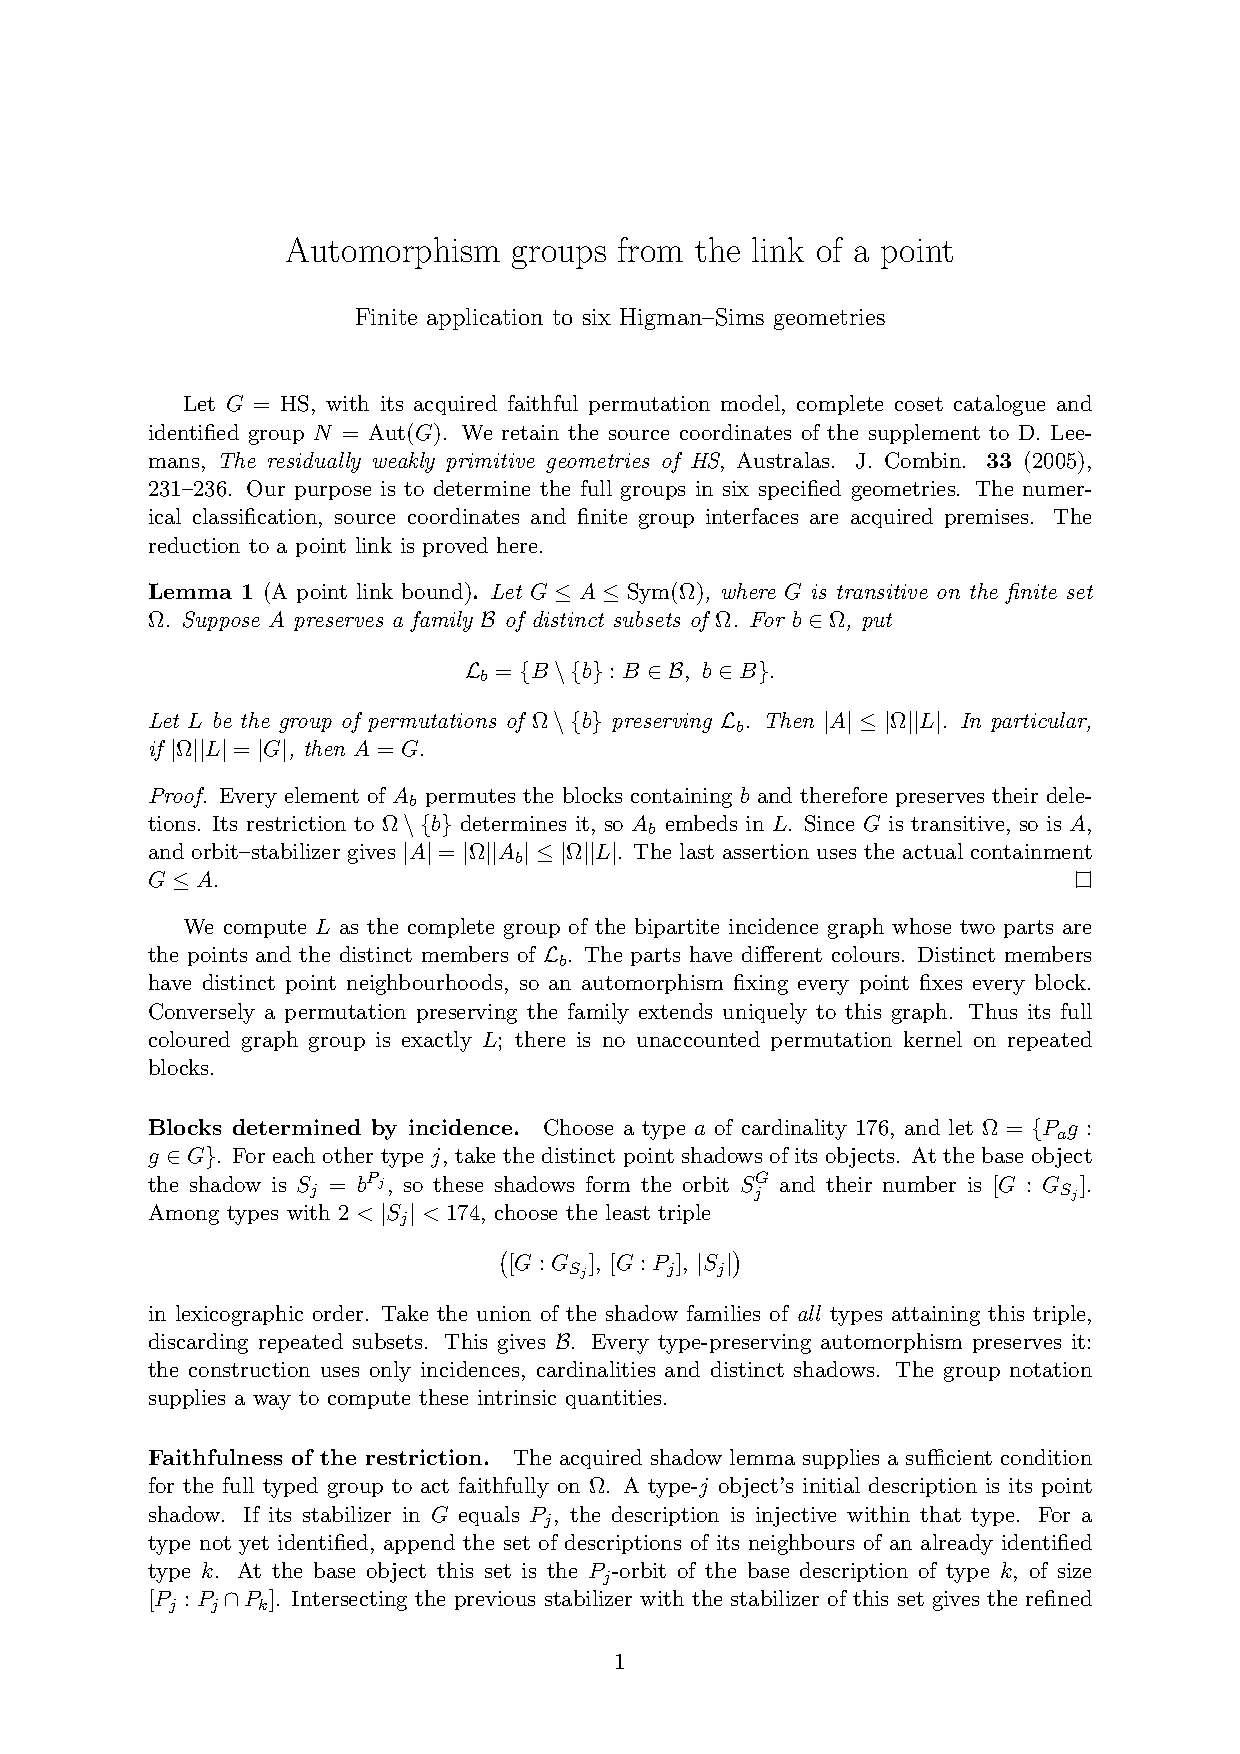
\includepdf[pages=-,pagecommand={},addtotoc={1,subsection,2,{Chapter 16: Six groups from point links},proof16}]{proofs/16.pdf}
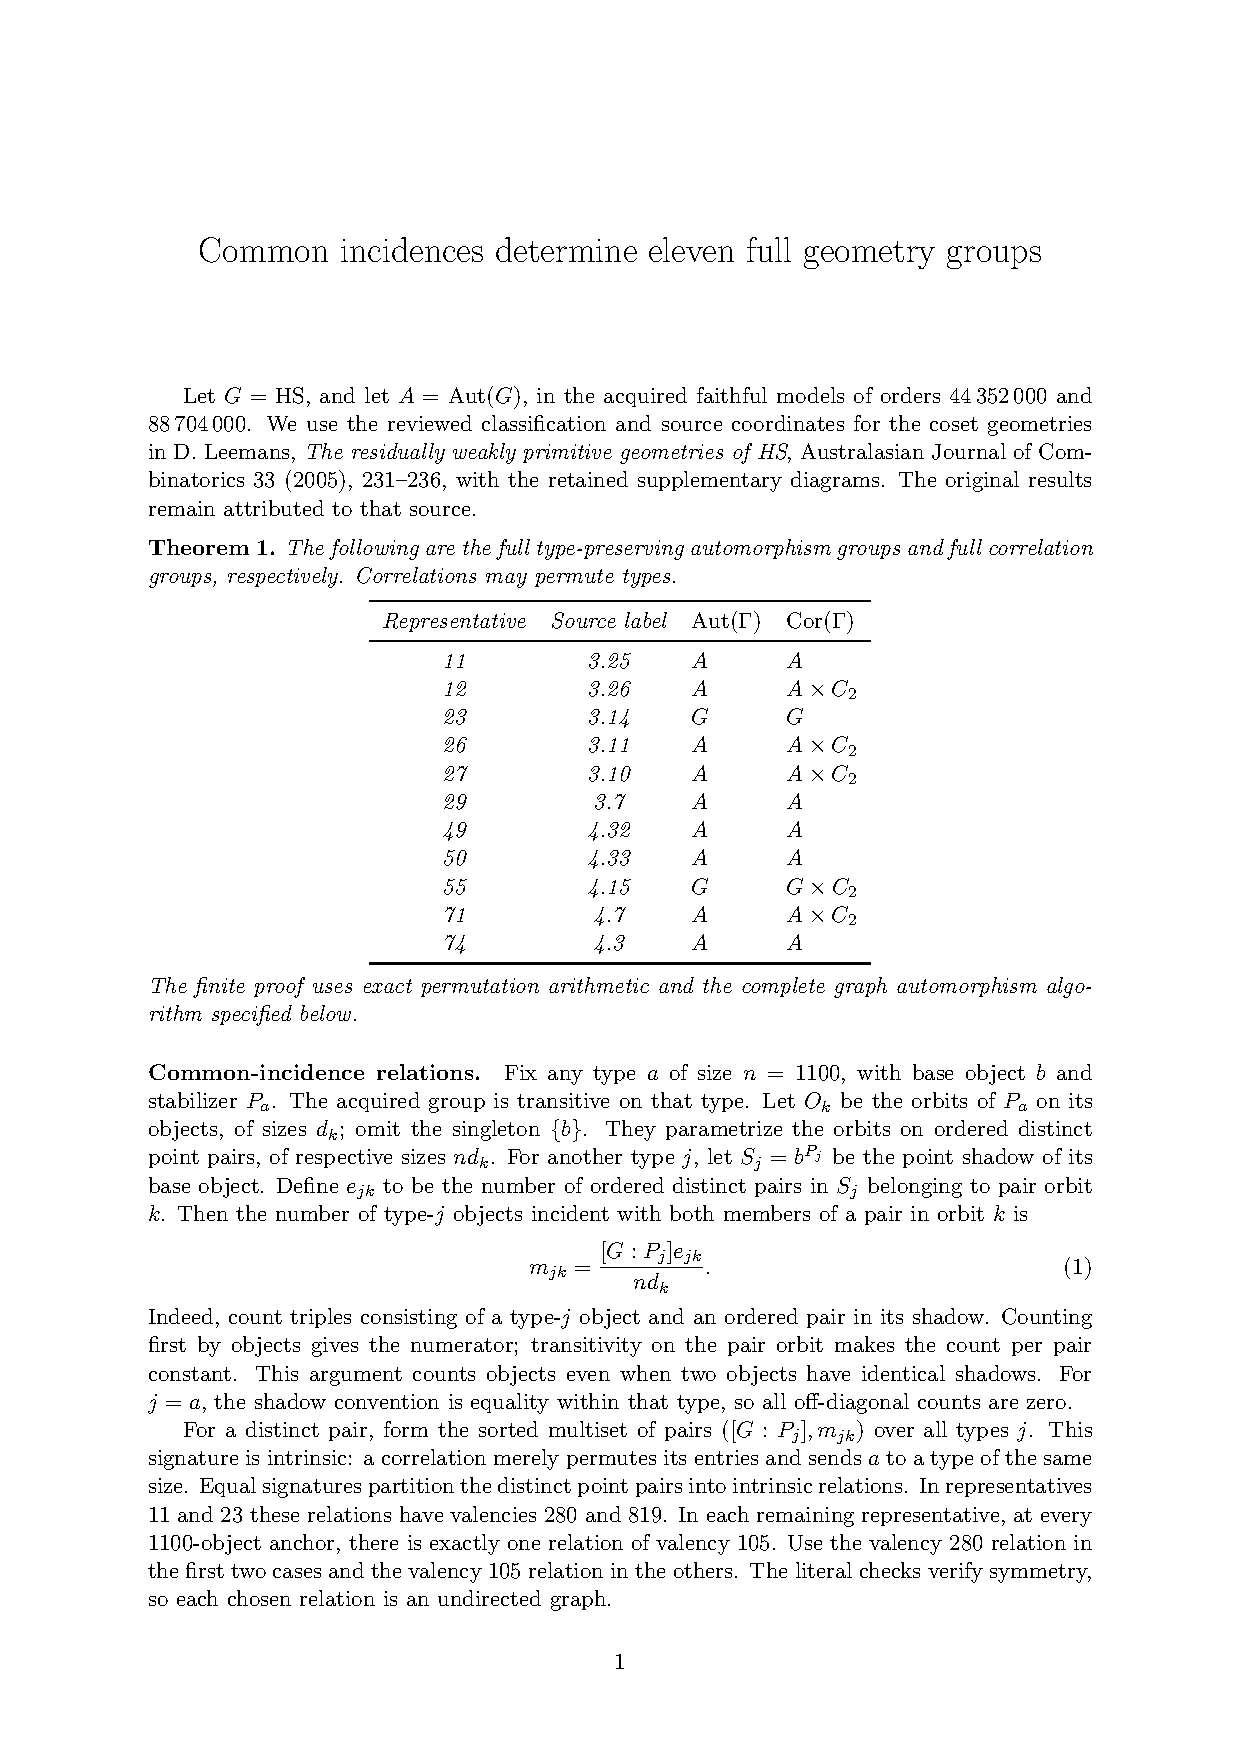
\includepdf[pages=-,pagecommand={},addtotoc={1,subsection,2,{Chapter 17: Eleven groups from common incidences},proof17}]{proofs/17.pdf}
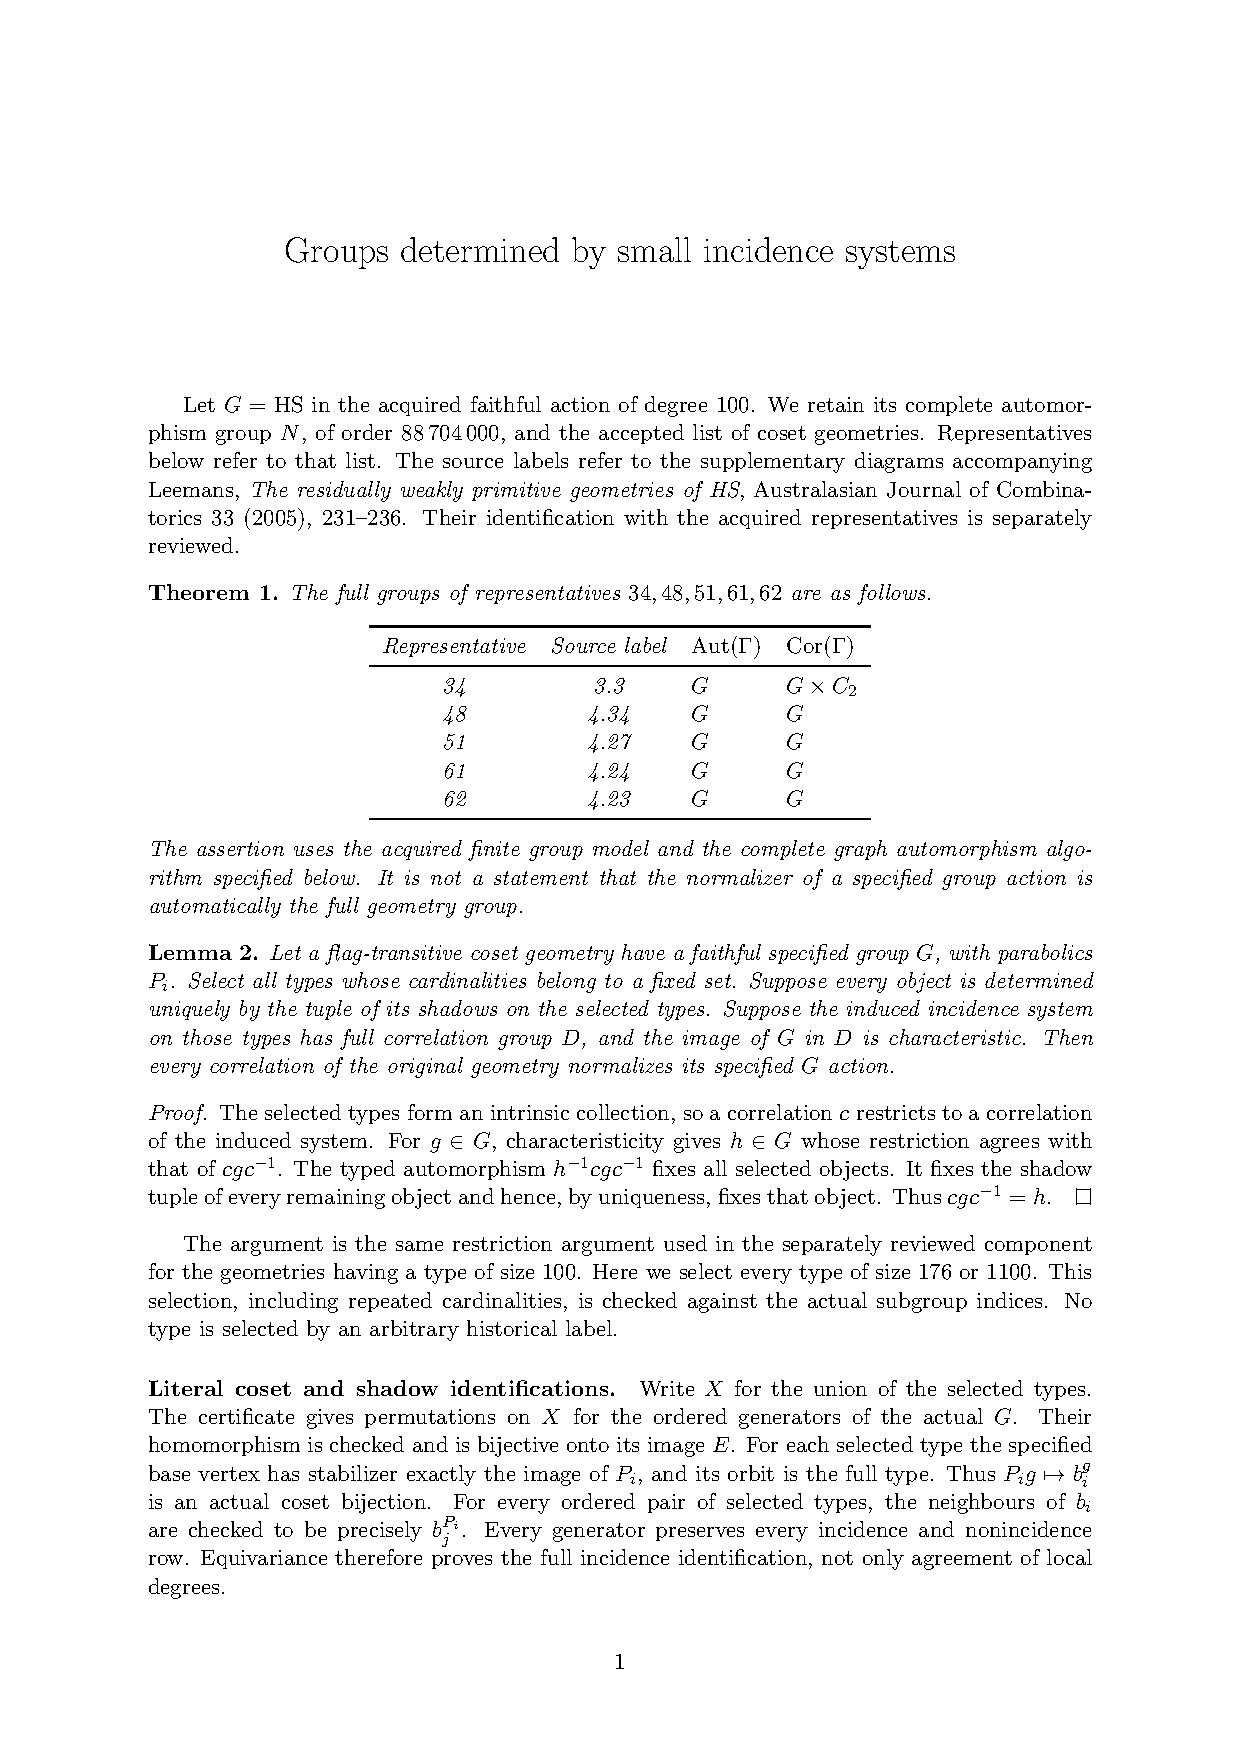
\includepdf[pages=-,pagecommand={},addtotoc={1,subsection,2,{Chapter 18: Five groups from small incidence systems},proof18}]{proofs/18.pdf}
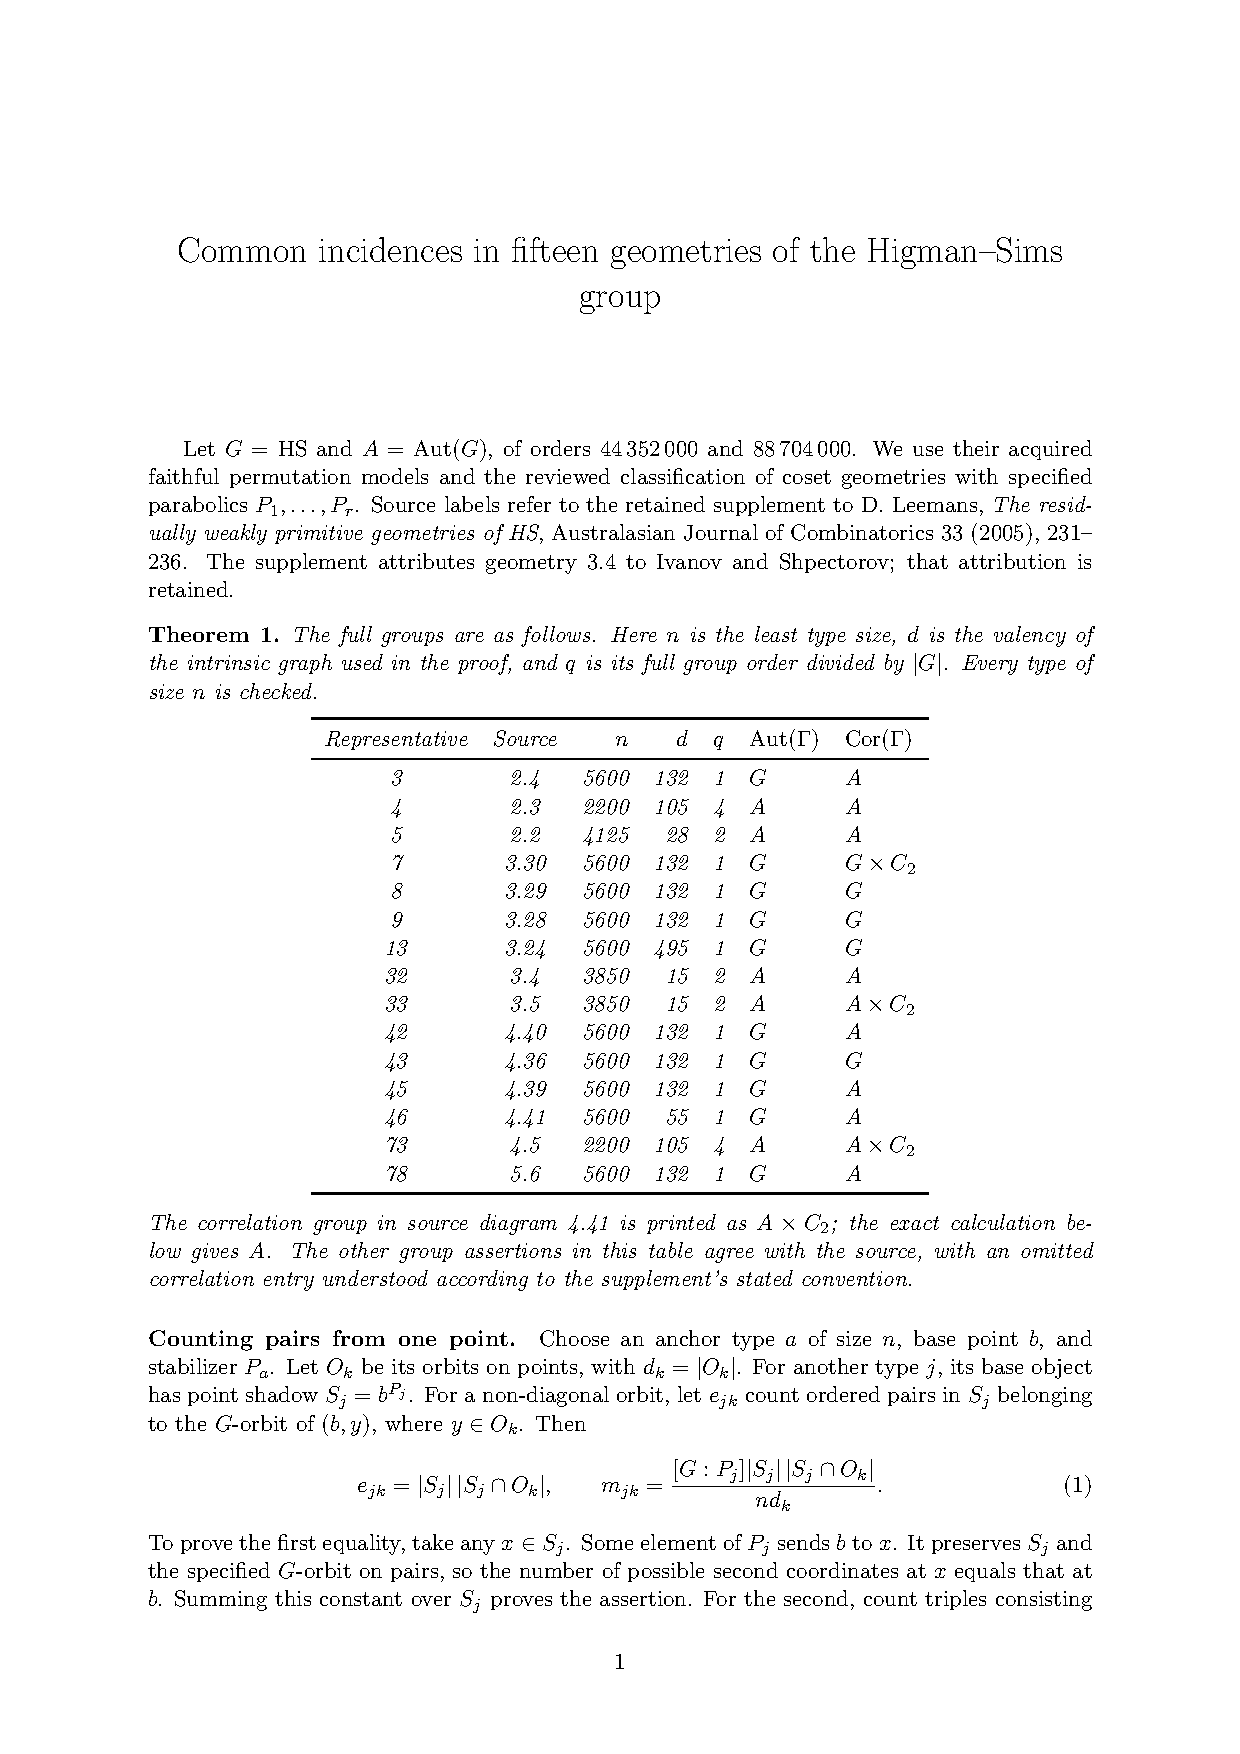
\includepdf[pages=-,pagecommand={},addtotoc={1,subsection,2,{Chapter 19: Fifteen groups from larger point actions},proof19}]{proofs/19.pdf}
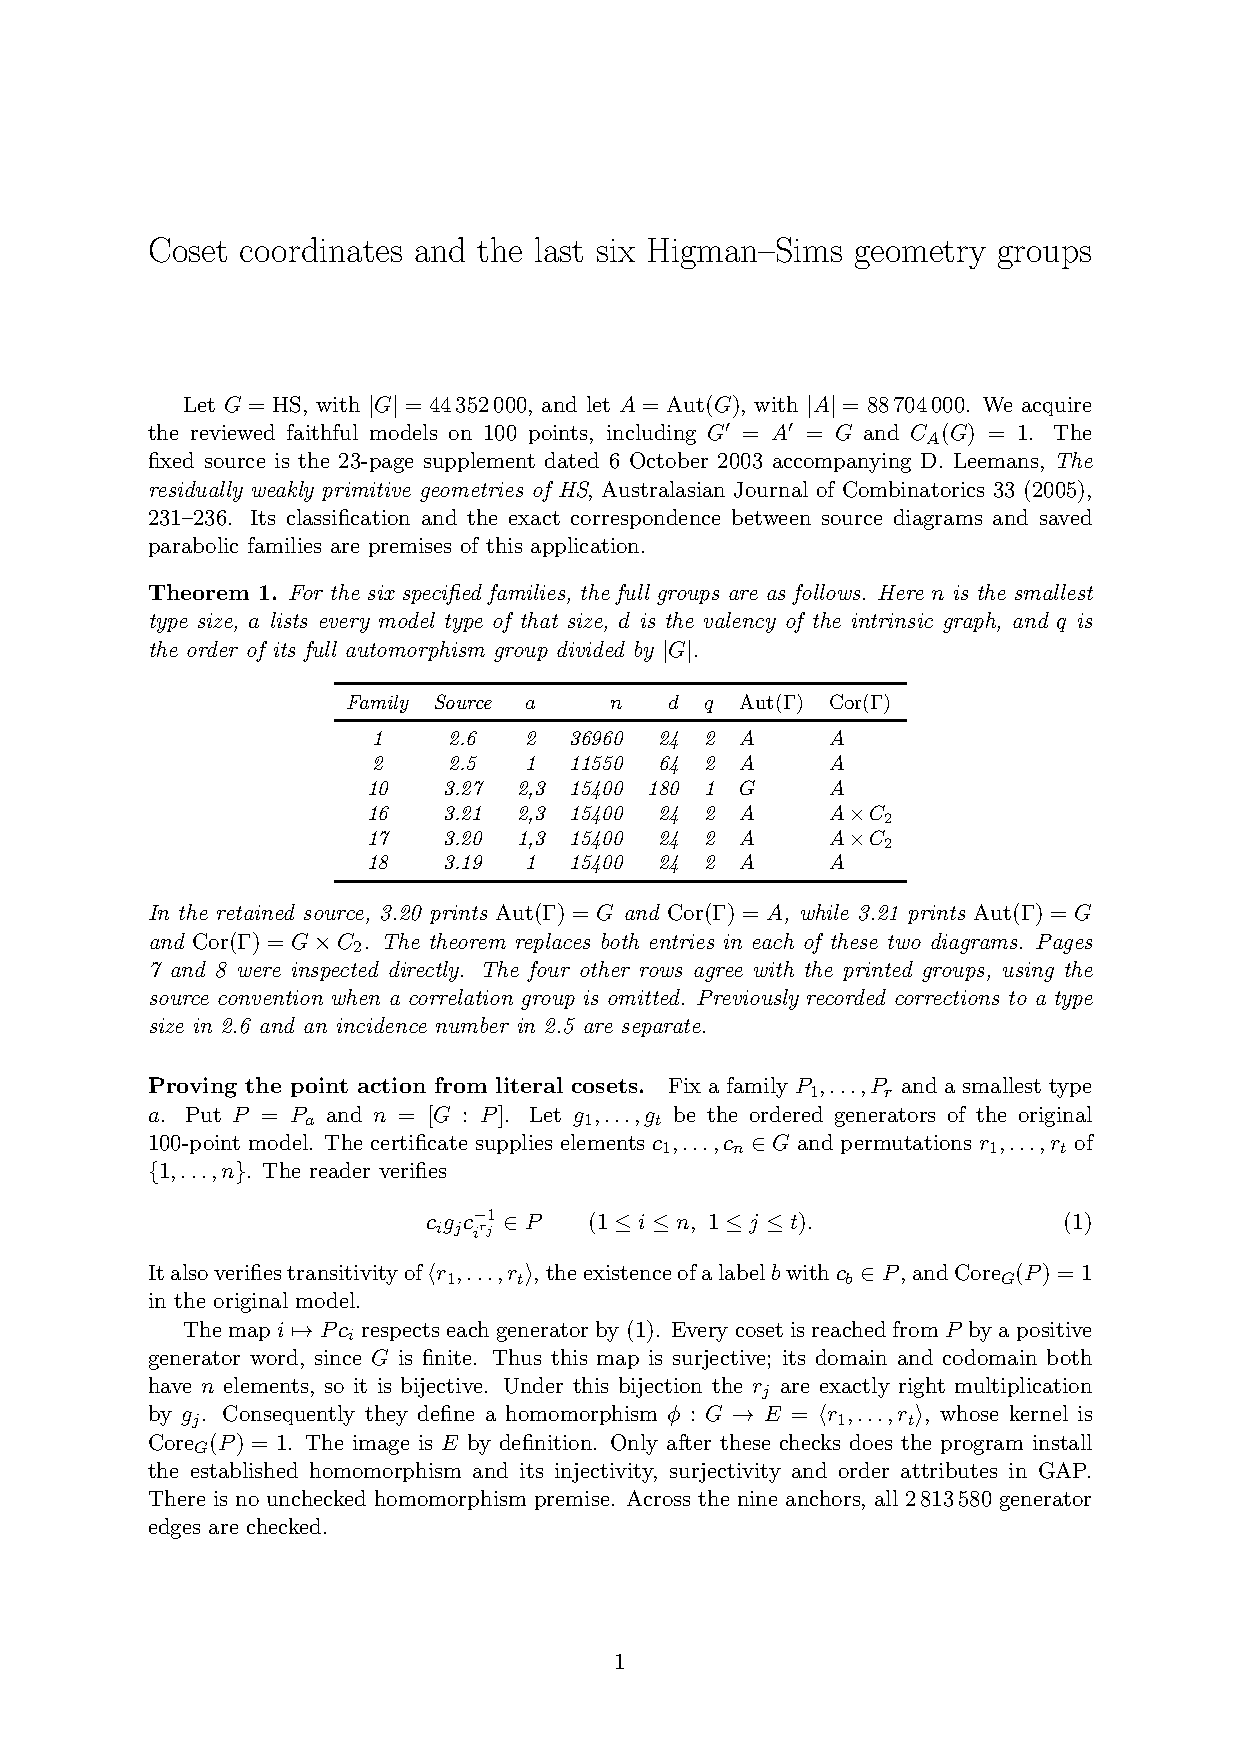
\includepdf[pages=-,pagecommand={},addtotoc={1,subsection,2,{Chapter 20: The last six geometry groups},proof20}]{proofs/20.pdf}
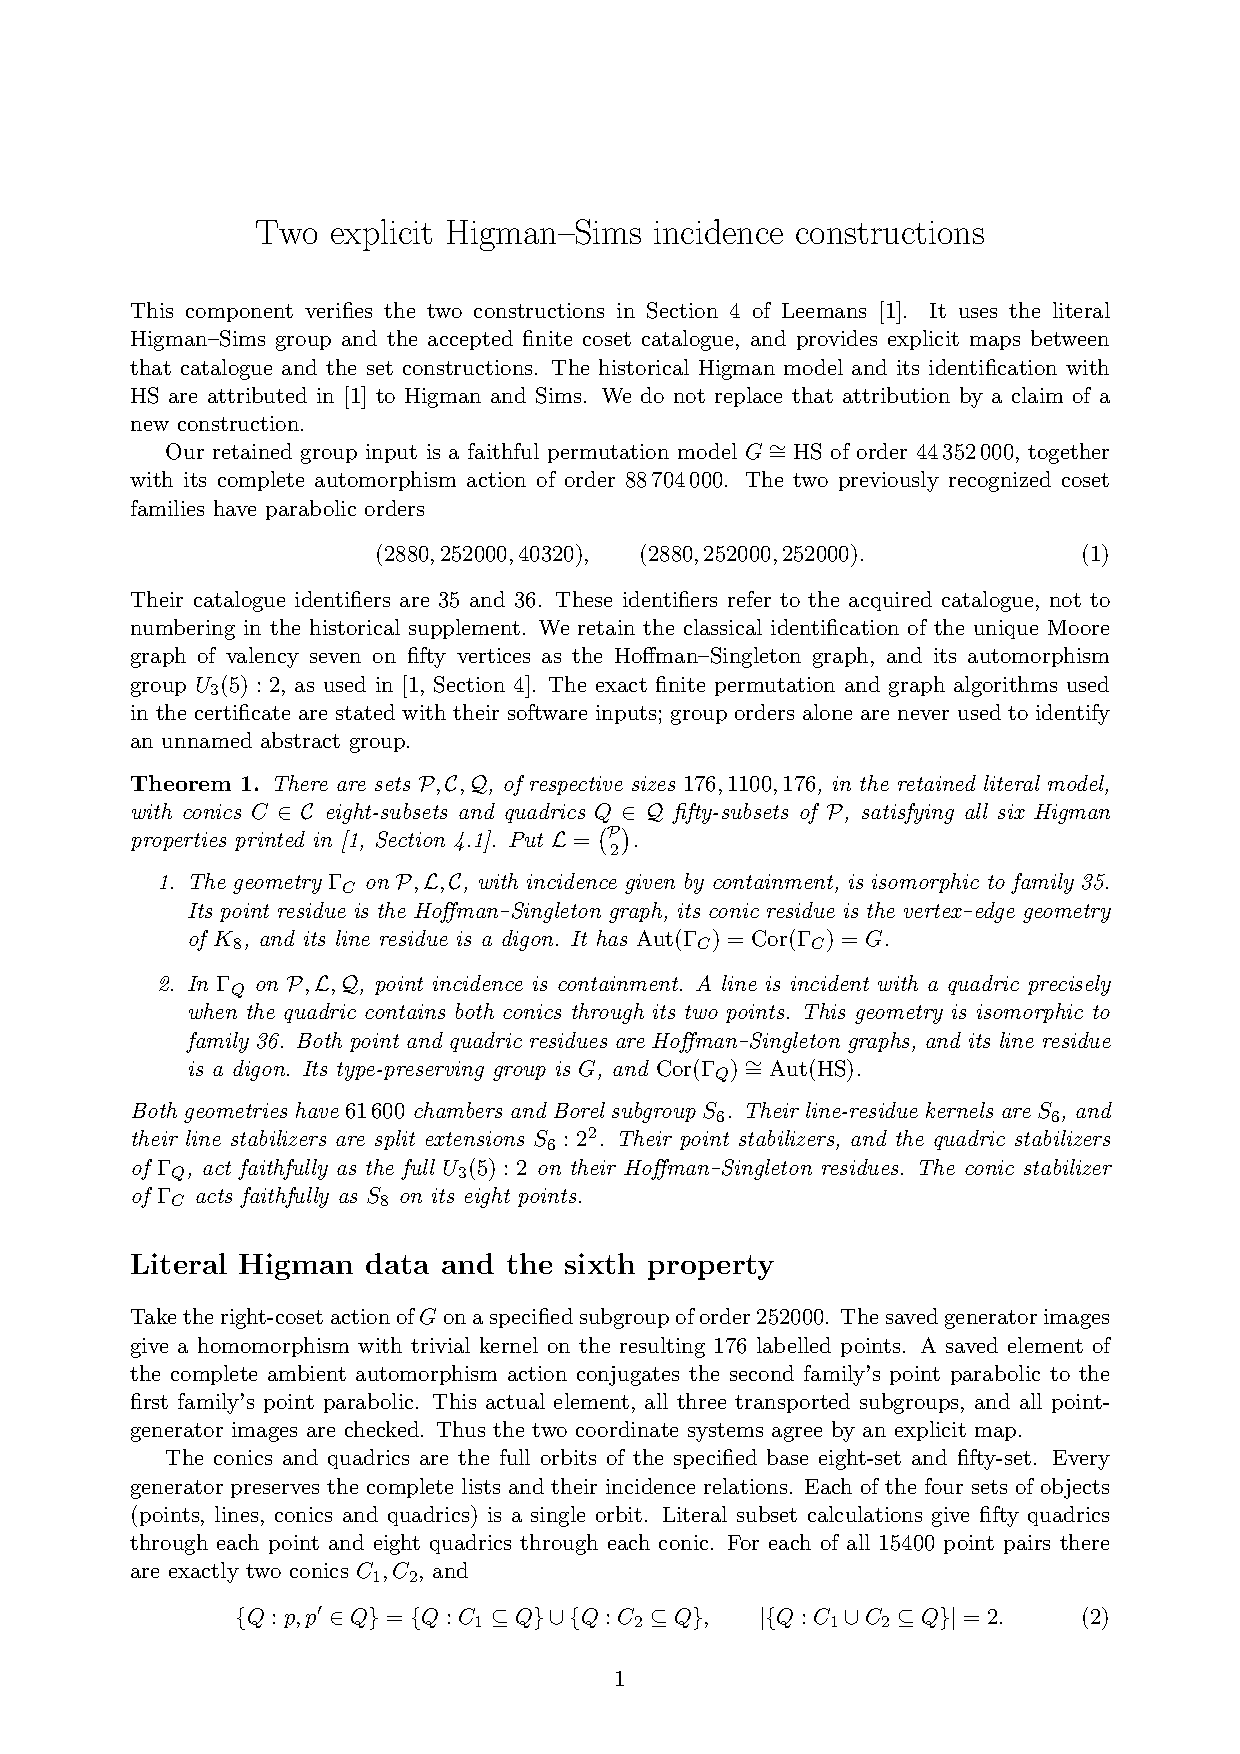
\includepdf[pages=-,pagecommand={},addtotoc={1,subsection,2,{Chapter 21: The two Hoffman--Singleton constructions},proof21}]{proofs/21.pdf}
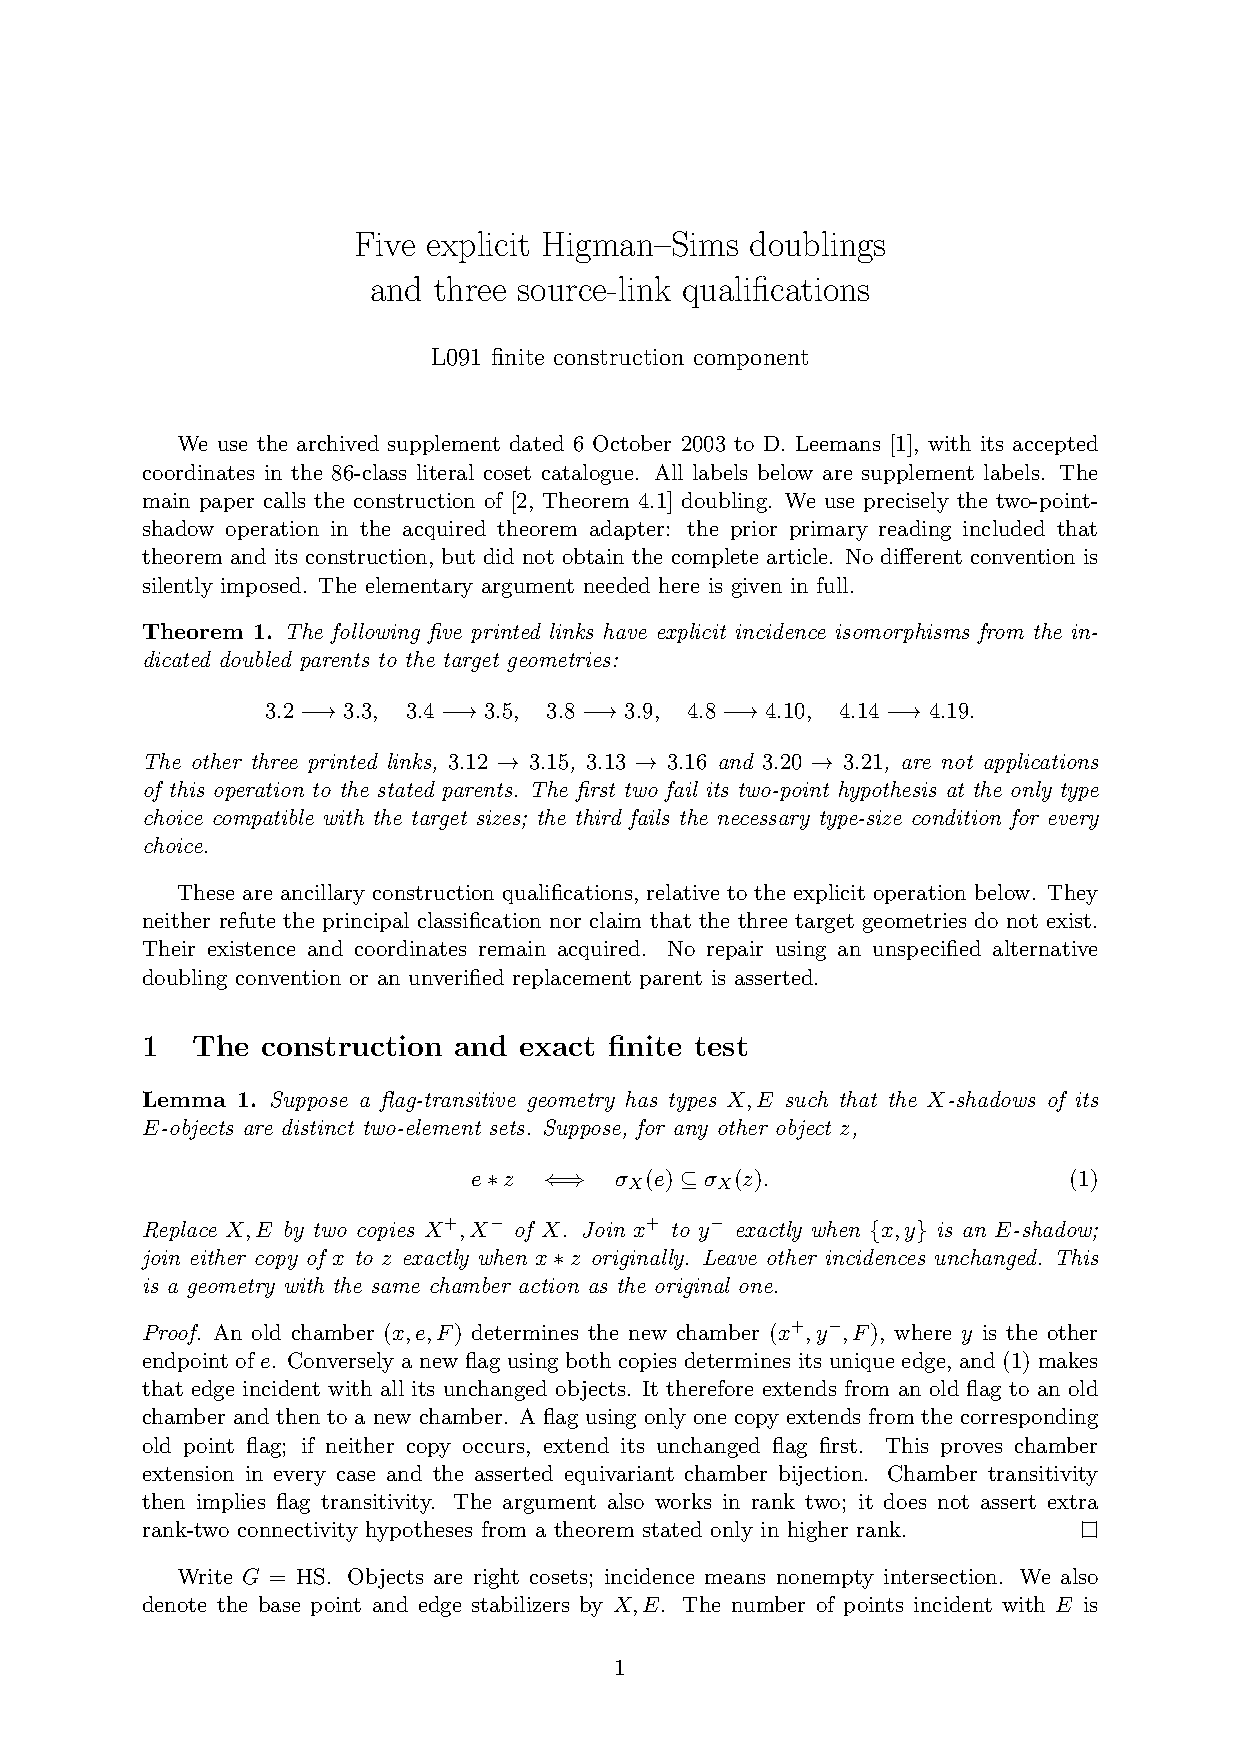
\includepdf[pages=-,pagecommand={},addtotoc={1,subsection,2,{Chapter 22: Five doublings and three qualifications},proof22}]{proofs/22.pdf}
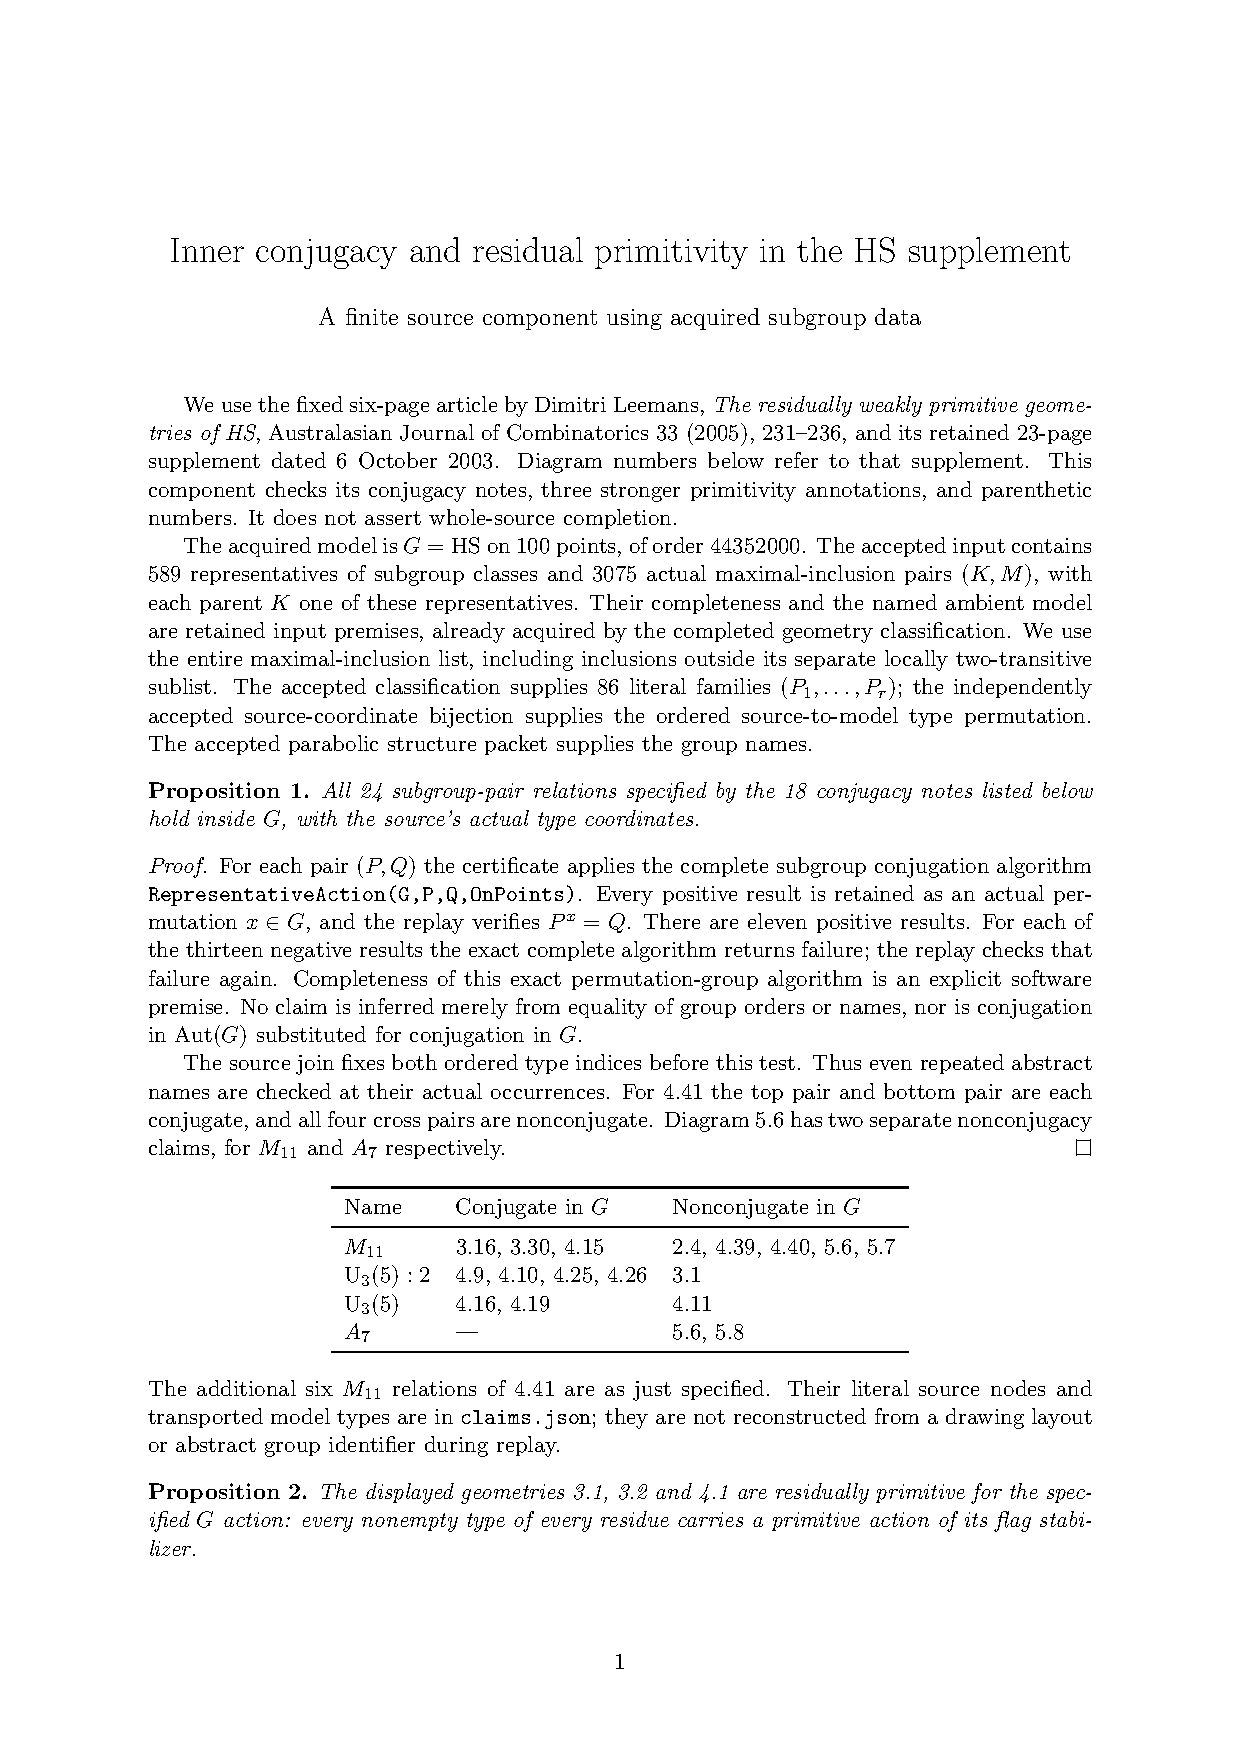
\includepdf[pages=-,pagecommand={},addtotoc={1,subsection,2,{Chapter 23: Conjugacy, primitivity and multiplicity annotations},proof23}]{proofs/23.pdf}
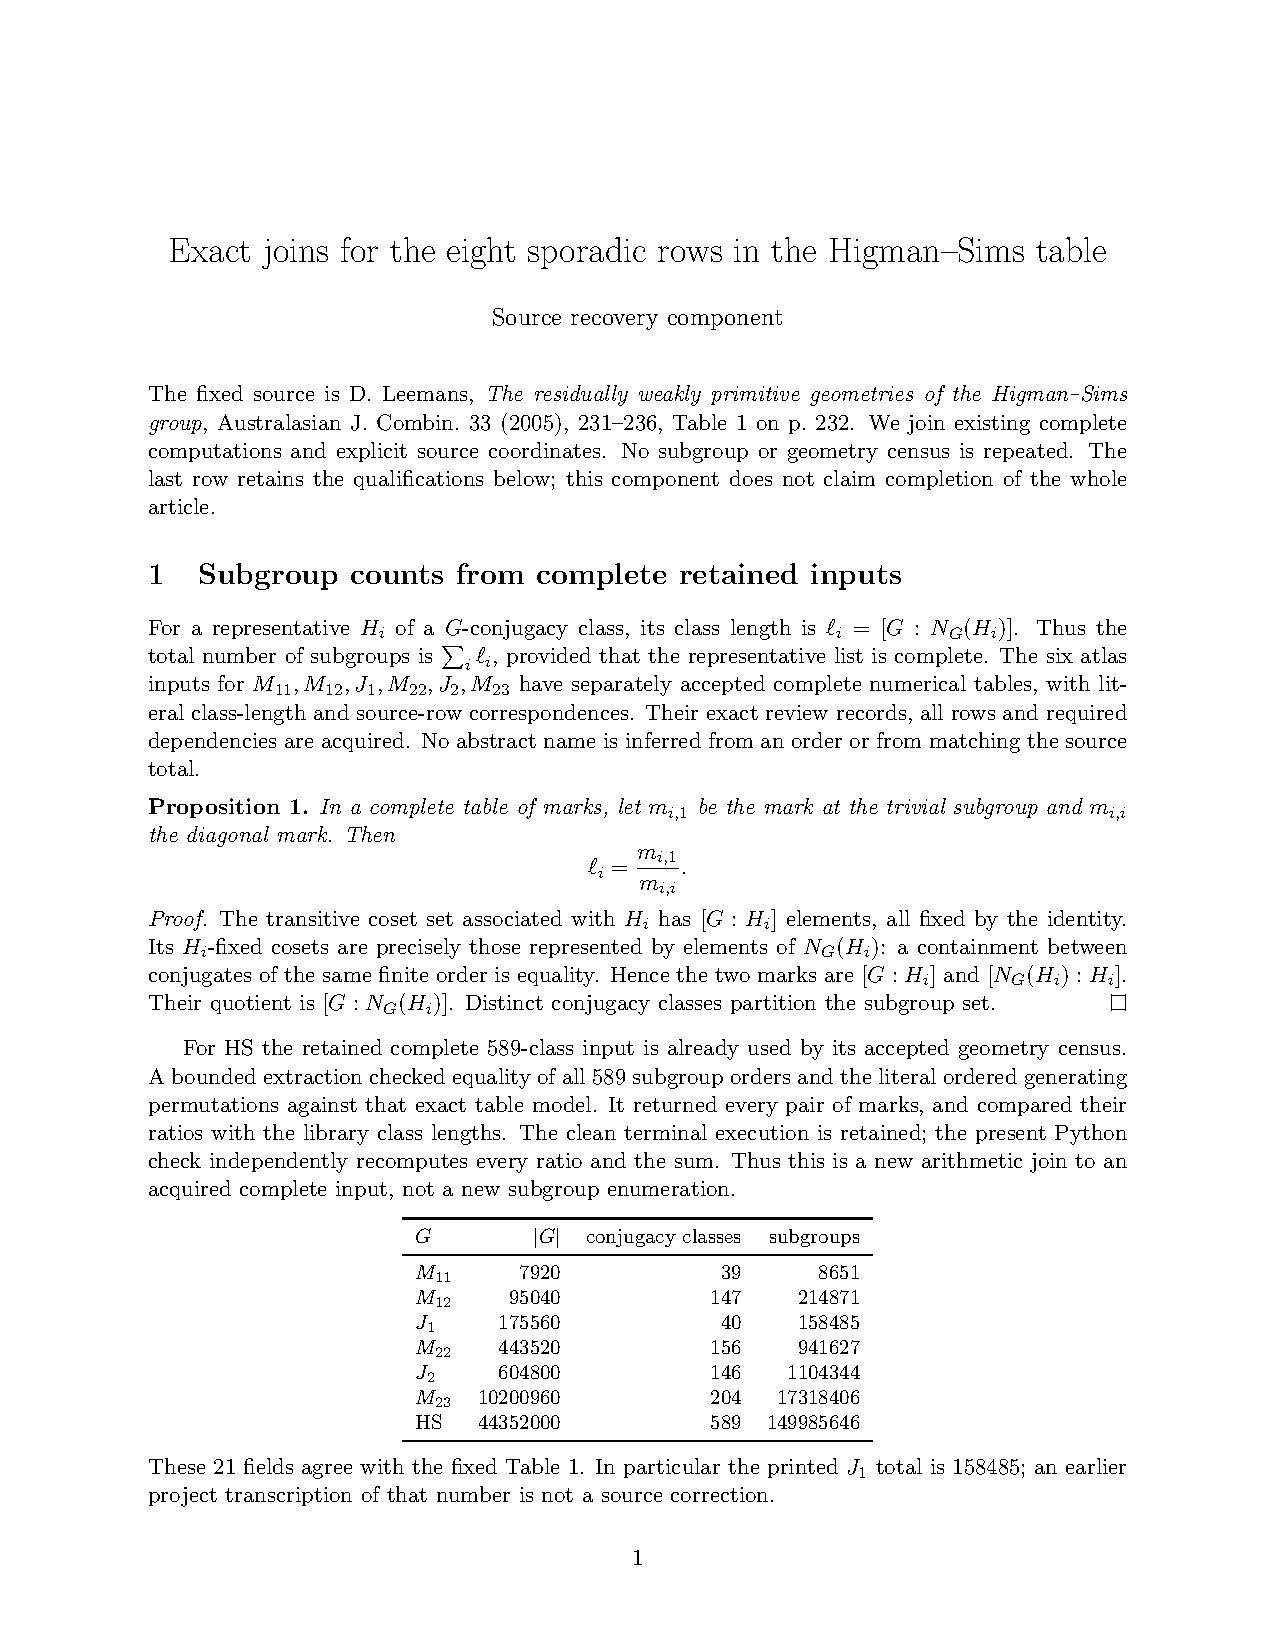
\includepdf[pages=-,pagecommand={},addtotoc={1,subsection,2,{Chapter 24: The first seven comparison rows},proof24}]{proofs/24.pdf}
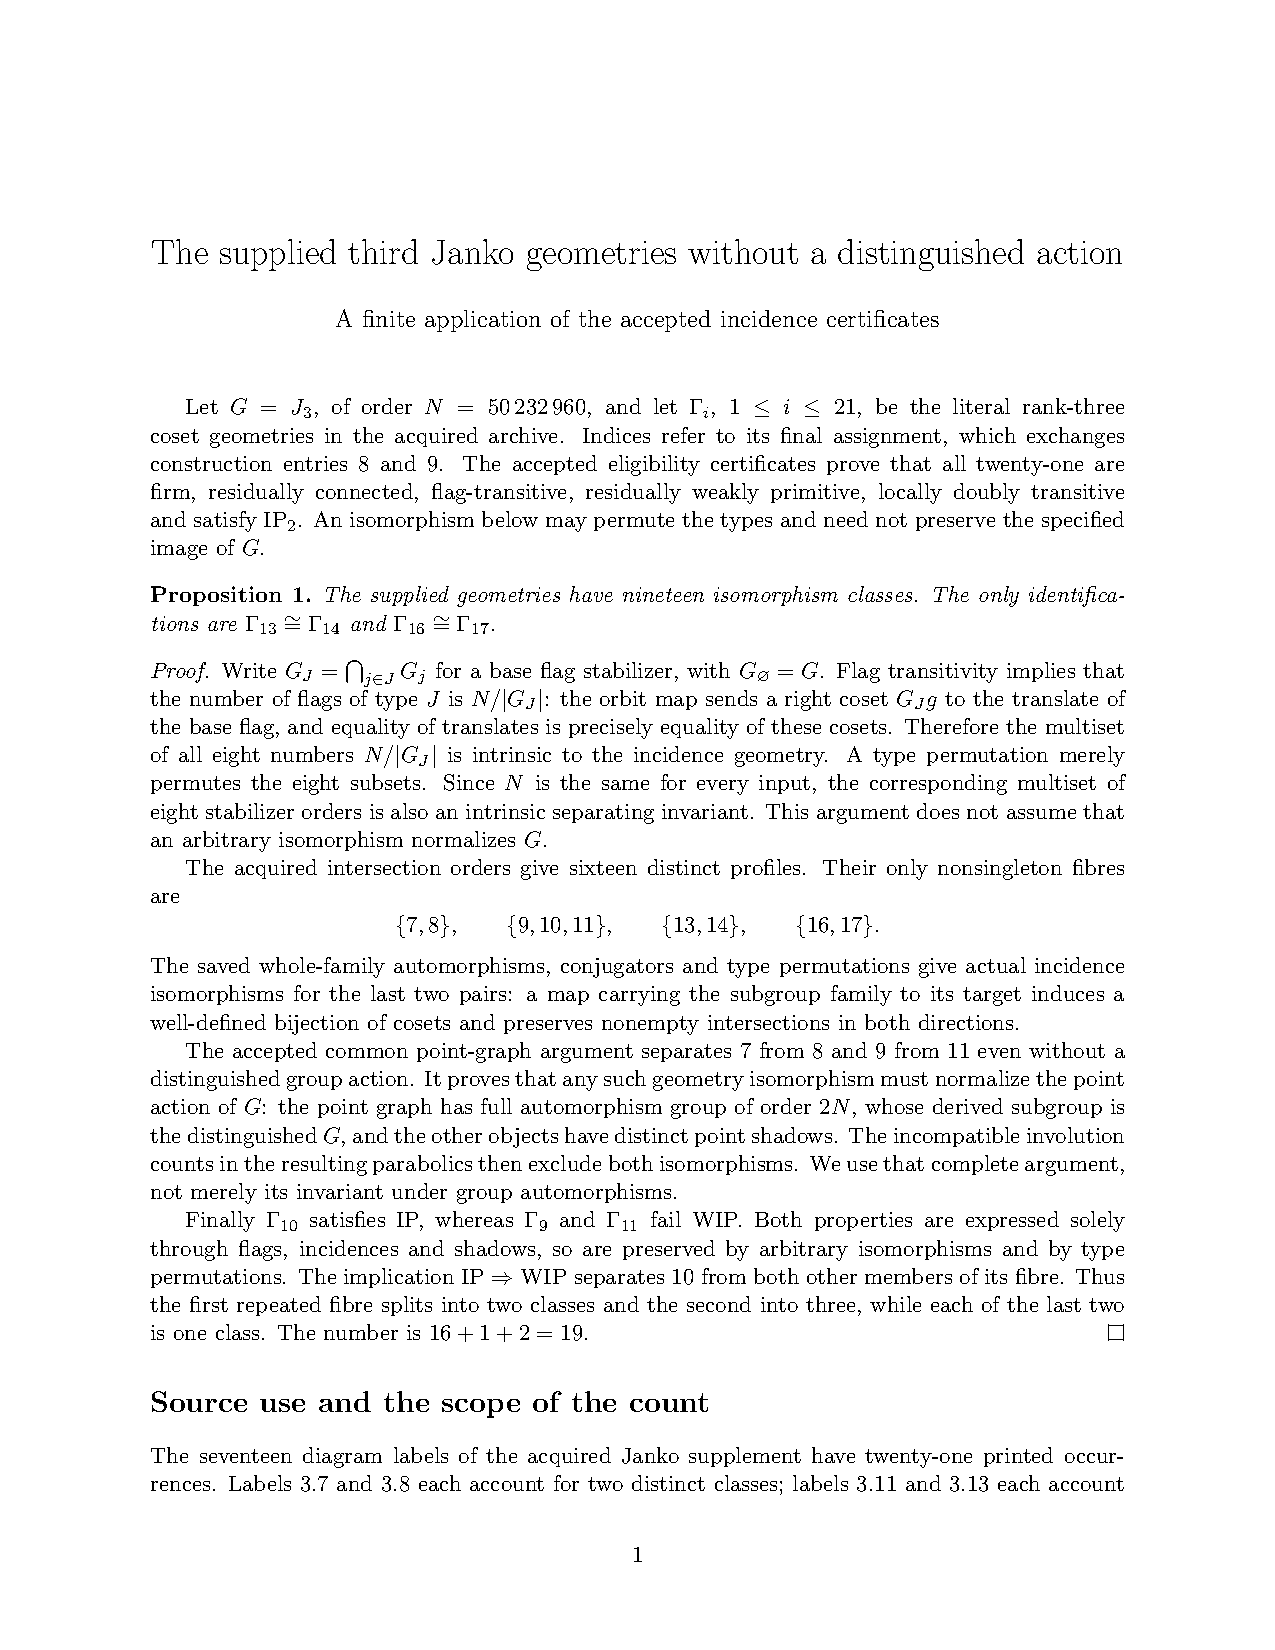
\includepdf[pages=-,pagecommand={},addtotoc={1,subsection,2,{Chapter 25: The nineteen supplied Janko classes},proof25}]{proofs/25.pdf}
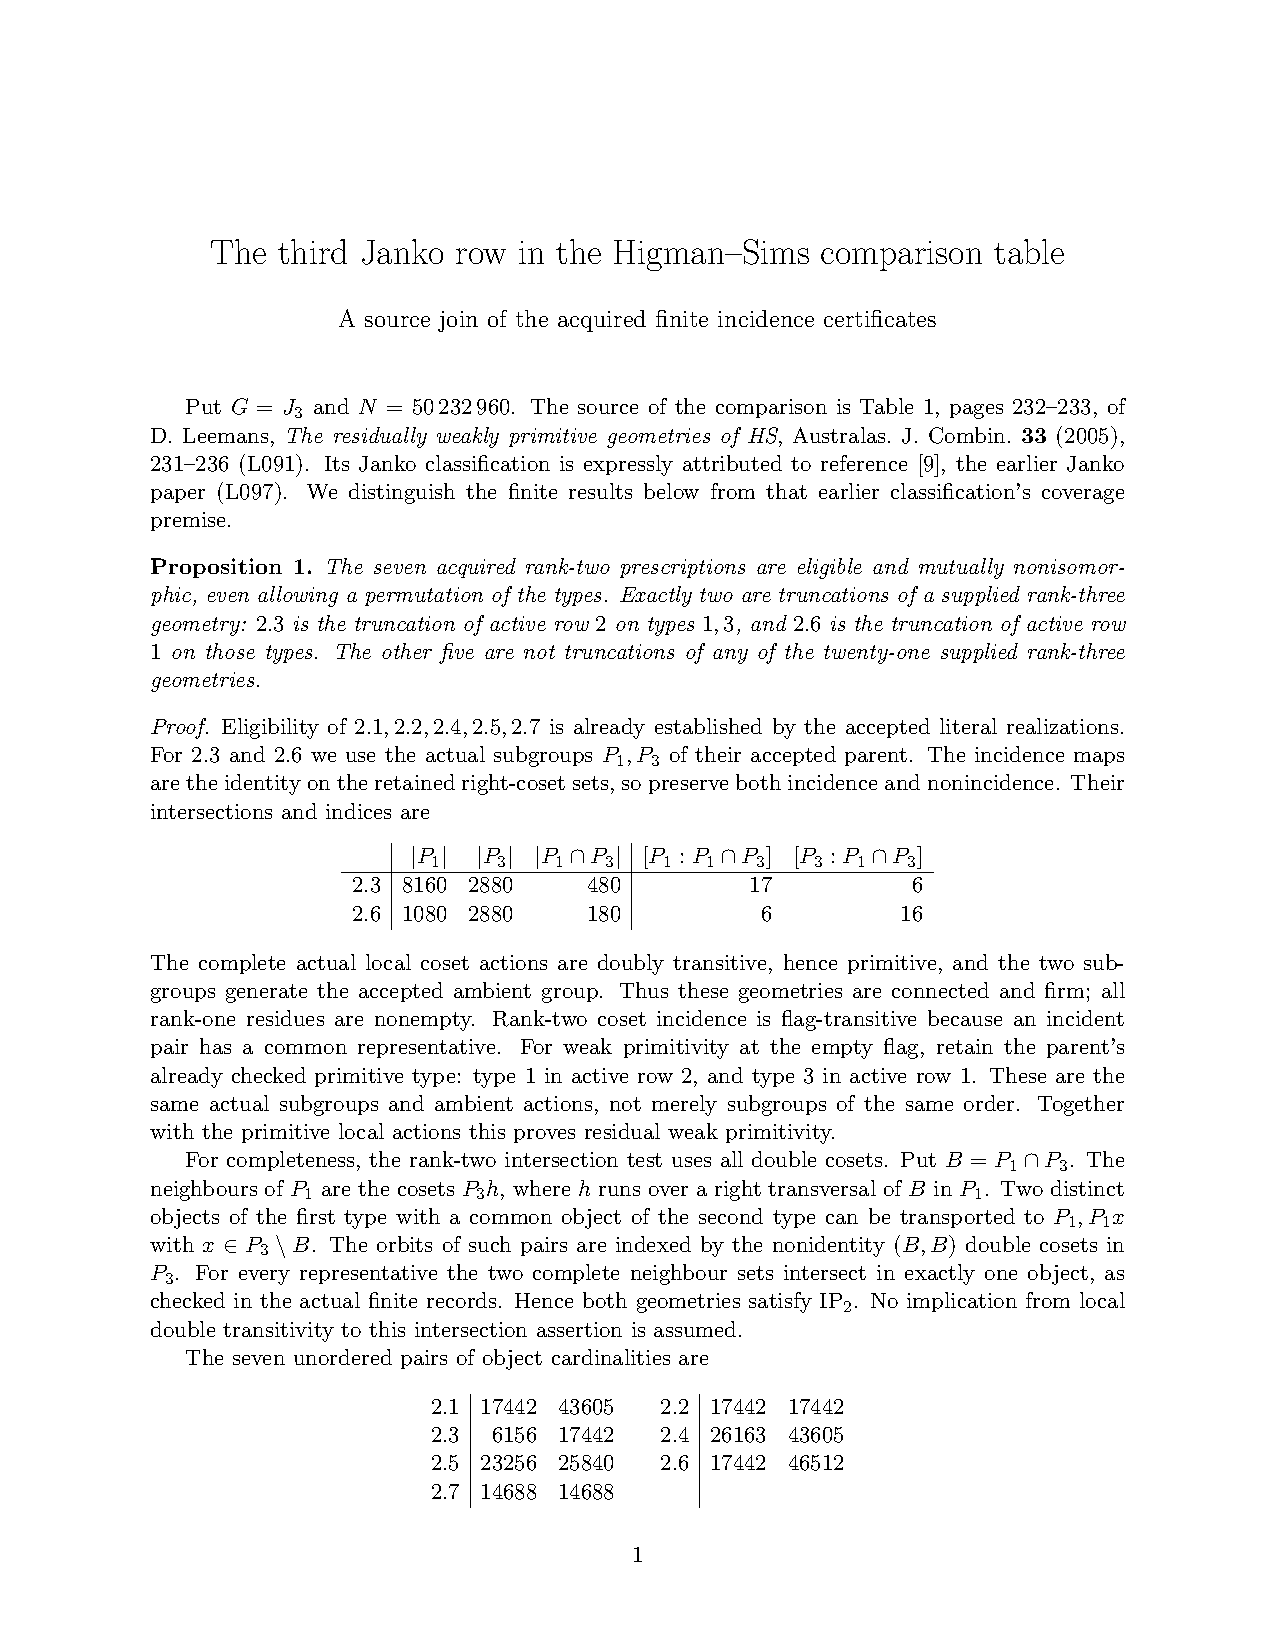
\includepdf[pages=-,pagecommand={},addtotoc={1,subsection,2,{Chapter 26: The final Janko comparison join},proof26}]{proofs/26.pdf}
\end{document}
